% Also note that the "draftcls" or "draftclsnofoot", not "draft", option
% should be used if it is desired that the figures are to be displayed in
% draft mode.
%
\documentclass[conference]{IEEEtran}
% Add the compsoc option for Computer Society conferences.

% Some very useful LaTeX packages include:
% (uncomment the ones you want to load)

\usepackage{cite}
\ifCLASSINFOpdf
   \usepackage[pdftex]{graphicx}
  % declare the path(s) where your graphic files are
   \graphicspath{{Images/}}
  % and their extensions so you won't have to specify these with
  % every instance of \includegraphics
   \DeclareGraphicsExtensions{.pdf,.jpeg,.png}
\else
  % or other class option (dvipsone, dvipdf, if not using dvips). graphicx
  % will default to the driver specified in the system graphics.cfg if no
  % driver is specified.
  % \usepackage[dvips]{graphicx}
  % declare the path(s) where your graphic files are
  % \graphicspath{{../eps/}}
  % and their extensions so you won't have to specify these with
  % every instance of \includegraphics
  % \DeclareGraphicsExtensions{.eps}
\fi
% graphicx was written by David Carlisle and Sebastian Rahtz. It is
% required if you want graphics, photos, etc. graphicx.sty is already
% installed on most LaTeX systems. The latest version and documentation
% can be obtained at: 
% http://www.ctan.org/tex-archive/macros/latex/required/graphics/
% Another good source of documentation is "Using Imported Graphics in
% LaTeX2e" by Keith Reckdahl which can be found at:
% http://www.ctan.org/tex-archive/info/epslatex/
%
% latex, and pdflatex in dvi mode, support graphics in encapsulated
% postscript (.eps) format. pdflatex in pdf mode supports graphics
% in .pdf, .jpeg, .png and .mps (metapost) formats. Users should ensure
% that all non-photo figures use a vector format (.eps, .pdf, .mps) and
% not a bitmapped formats (.jpeg, .png). IEEE frowns on bitmapped formats
% which can result in "jaggedy"/blurry rendering of lines and letters as
% well as large increases in file sizes.
%
% You can find documentation about the pdfTeX application at:
% http://www.tug.org/applications/pdftex


% correct bad hyphenation here
\hyphenation{op-tical net-works semi-conduc-tor}

\usepackage{url}
\usepackage[table, svgnames]{xcolor} 
\usepackage{color}
\usepackage{siunitx}

\usepackage{dcolumn}
\newcolumntype{Y}{D..{6.4}}

\begin{document}
%
% paper title
% can use linebreaks \\ within to get better formatting as desired
% Do not put math or special symbols in the title.

\title{Tool Support for Questions Developers Ask About Security Vulnerabilities}
% What Questions Do Developers Ask When Reasoning about the Security of Their Code? Building Tools that Answer Developers' Questions about Security Vulnerabilities?

% author names and affiliations
% use a multiple column layout for up to three different
% affiliations
\author{\IEEEauthorblockN{Justin Smith, Brittany Johnson, and Emerson Murphy-Hill}
\IEEEauthorblockA{North Carolina State University\\
Raleigh, NC 27606}
\and
\IEEEauthorblockN{Bill Chu and Heather Richter Lipford}
\IEEEauthorblockA{University of North Carolina at Charlotte\\
Charlotte, NC 28223 \\
\{billchu, heather.lipford\}@uncc.edu
}}

\maketitle

% As a general rule, do not put math, special symbols or citations
% in the abstract
\begin{abstract}

Program analysis tools should help developers answer the security-relevant questions; to design tools that help developers answer their questions, we must first understand what questions they ask.
However, we lack a catalog and categorization of such questions in relation to security. 
We attempted to build this categorized catalog by conducting a laboratory experiment with novice and experienced software developers, observing their interactions with security vulnerabilities in iTrust, a Java medical records software system.
Results of our study have several implications for program analysis tools aiming to help developers assess security vulnerabilities in their code, such as providing support for reasoning about the different possible attacks that could stem from a given security vulnerability.



\end{abstract}
% no keywords

% For peer review papers, you can put extra information on the cover
% page as needed:
% \ifCLASSOPTIONpeerreview
% \begin{center} \bfseries EDICS Category: 3-BBND \end{center}
% \fi
%
% For peerreview papers, this IEEEtran command inserts a page break and
% creates the second title. It will be ignored for other modes.
\IEEEpeerreviewmaketitle



\section{Introduction}
% no \IEEEPARstart


Software developers are a critical part of making software secure. 
When there is a security fault in a software system, it is up to the developers to determine the best way to remove the vulnerability and ensure proper function of the system in the future.
There are a variety of ways developers can learn about, assess, and fix insecure code, such as peer interactions or usage of tools.
It is particularly important that effectives tools exist for secure systems, as security vulnerabilities are more likely to cause incidents that affect company budgets as well as end users~\cite{chen2002mops}. 

Static analysis tools are made available to help developers detect potential security flaws in their code. 
One of example of such a tool is FindBugs, a static analysis tool for finding potential defects in software code.~\footnote{findbugs.sourceforge.net} 
FindBugs is able to report various potential security defects, such as SQL injection and cross site scripting.  % more specific example? figure? 
There is also an extension for FindBugs, called Find Security Bugs (FSB), that focuses its reporting efforts specifically on security vulnerabilities~\footnote{\url{h3xstream.github.io/find-sec-bugs/}}.
Other tools, such as CodeSonar~\footnote{\url{http://www.grammatech.com/codesonar}} and Coverity~\footnote{\url{http://www.coverity.com/}}, can also be used to detect and remove potential security vulnerabilities.

% maybe connect back to example.
Unfortunately, however, research suggests that many developers may not be using these tools; part of this reason for this is that they have difficulty interpreting the output~\cite{johnson2013don}. 
Part of this difficulty for developers building secure systems stems from the hard to answer questions developers have about the security of their code~\cite{latoza2010hard}.
Though not the goal of their work, many researchers have taken the findings of LaToza and colleagues and been able to work towards improving the state-of-the-art for program analysis tools~\cite{kononenko2012automatically, servant2012history, yoon2013visualization}. 
Because LaToza's work only addresses security questions in passing and does not focus on the process of assessing potential security vulnerabilities, we do not have such a collection of questions to use to build better, more usable tools for security.
Our work extends existing work to security by providing a similar catalog of the questions that developers ask when assessing potential security vulnerabilities.

In this paper, we report a study conducted to create a better understanding of the information developers seek with using static analysis tools to identify and assess security vulnerabilities in code.
We conducted a laboratory experiment with 10 developers familiar with the iTrust software system.~\footnote{\url{http://agile.csc.ncsu.edu/iTrust/wiki/doku.php?id=start}} 
We observed each developer as they assessed potential security vulnerabilities reported by FSB and report the kinds of questions they asked while doing so along with the strategies they used, if any, to answer them.
Using a card sort methodology, we sorted the 559 questions into 17 categories. 

Our work makes three contributions. 
First, we present a list of questions that software developers ask when examining the security of their code.
Second, based on our observations, we discuss the strategies that developers use to answer some of their questions.
Finally, we evaluate the existing tool support for answering security-related questions.

The remainder of the paper is organized as follows. 
In Section~\ref{sec:rw}, we discuss previous work related to our own. 
Section~\ref{sec:meth} outlines the methodology we used to conduct our study and analyze our data. 
Next, we discuss the findings of our study in four parts. 
Section~\ref{sec:results-vaf} reports findings related to vulnerabilities, attacks and fixes. 
Section~\ref{sec:results-ca} discusses questions pertaining to the code and the application in which the code resides.
Section~\ref{sec:results-i} reports findings pertaining the individuals and their thought processes.
Section~\ref{sec:results-pss} reports questions surrounding resources for solving the problem.
Each section of findings includes observations made and implications for tool design that can be drawn based on these observations. 
Finally, we conclude the paper with a discussion of future work~\ref{sec:fw}.






%Figure, high res, png or vector (pdf)

\section{Related Work}
\label{sec:rw}

We have organized the related work into three sections. Section \ref{evaluation} outlines the predominant approaches researchers use to evaluate security tools. 
Section \ref{understanding} surveys the work done to facilitate developers' understanding of code, and section \ref{questions} references similar studies that have explored the questions developers ask when modifying, understanding, or debugging their code.

\subsection{Evaluation of Techniques}
\label{evaluation}
Developers use several techniques and tools to help secure their systems.
Using a variety of metrics, many studies have assessed the effectiveness of the tools and techniques developers use to find and remove vulnerabilities from their code~\cite{martin2005finding, austin2011one, livshits2005finding}.  

Much research has evaluated the effectiveness of tools and techniques based on their false positive rates and how many vulnerabilities they detect~\cite{jovanovic2006pixy, austin2011one, dukes2013case}. 
Jovanovic and colleagues attempt to address the problem of vulnerabilities in web applications by implementing and evaluating \textsc{Pixy}, a static analysis tool that detects cross-site scripting vulnerabilities in PHP scripts~\cite{jovanovic2006pixy}. 
They considered their tool effective because of its low false positive rate (50\%) and its ability to find vulnerabilities previously unknown. 
Similarly, Livshits and Lam evaluated their own approach to static analysis for detecting security vulnerabilities; the static analyzers used are created from specifications provided by the user~\cite{livshits2005finding}. 
They also found their tool to be effective because it had a low false positive rate. 

Austin and Williams compared the effectiveness of four existing techniques for discovering security vulnerabilities: systematic and exploratory manual  penetration testing, static analysis, and automated penetration testing~\cite{austin2011one}. 
Comparing the four approaches based on number of vulnerabilities found, false positive rate, and efficiency, they reported that no one technique was capable of discovering every type of vulnerability. 
Dukes and colleagues conducted a case study comparing static analysis and manual testing techniques used to find security vulnerabilities~\cite{dukes2013case}. 
They found that the combination of manual testing and static analysis was most effective, because it found the most vulnerabilities.


These studies use various measures of effectiveness, such as false positive rates or vulnerabilities found by a tool, but none focus on how developers interact with the tool. 
Further, they do not evaluate whether the tools under study answer questions that developer have about the code or vulnerabilities. 
Unlike existing studies, our study explores the questions developers ask when attempting to understand the vulnerabilities in their code.

\subsection{Developer Understanding}
\label{understanding}
In non-security domains, research has shifted focus from the technical effectiveness of program analysis tools to usability~\cite{johnson2013don, ayewah2008using, khoo2008path}. 
These studies sought to evaluate how tools communicate information to developers and how a tool can enhance a developer's understanding of the code. 
Such studies examine proposed and existing approaches using various qualitative methods such as interviews and surveys. 

Some research surrounding tool effectiveness shifted focus from technical effectiveness of program analysis tools to usability~\cite{johnson2013don, ayewah2008using, khoo2008path}. 
The goal of these studies was to evaluate how tool designers can help developers cope with existing or proposed approaches, through comparison of proposed and existing approaches and various qualitative methods, such as interviews and surveys.

Ayewah, Pugh, and colleagues conducted a series of interviews and surveys, along with a controlled user study, in an attempt to better understand the practices and needs of developers when using the static analysis tool FindBugs~\cite{ayewah2008report, ayewah2008using}.

Khoo and colleagues focused their efforts on improving the user interface of existing tools by developing and evaluating \textsc{Path Projection}, a user interface toolkit to help developers navigate through and understand the errors in their code~\cite{khoo2008path}.

Johnson and colleagues conducted semi-structured interviews with professional developers to determine the reason developers have for using, and possibly not using, static analysis tools to find defects in their codes~\cite{johnson2013don}. 
Their findings suggest that one of the biggest reasons developers may have for not using tools to analyze their code is difficulty understanding the output provided. 

Layman and colleagues conducted a study with developers to explore the factors developers consider when deciding whether they will fix a defect or not~\cite{layman2007toward}. 
They found that, among other criteria considered, developers consider the description of the fault critical to assessing its importance. 
Based on their findings, they discuss design implications for automated fault detection tools.

These studies discuss the ability of developers to effectively use existing tools and ways to improve them, however, these studies do not focus on the information needs of developers when using static analysis tools in their code. 
The goal of our study is to identify the security-related questions developers ask when approaching security vulnerabilities so that tool designers understand the information requirements of security-minded developers.

\subsection{Answering Developer Questions}
\label{questions}
Several studies have explored the knowledge requirements of developers when coding.
Similar to our work, some existing studies focus on the questions developers ask to determine these knowledge requirements~\cite{latoza2010hard, latoza2010developers}.
In contrast, our study focuses specifically on the knowledge requirements of developers when assessing security vulnerabilities.


Much of the work on answering developer questions has occurred in the last decade. 
LaToza and Myers surveyed professional software developers to understand the questions developers ask during their daily coding activities, focusing on the hard to answer questions~\cite{latoza2010hard}. 
Futhermore, after observing developers in a lab study, they discovered that the questions developers ask tend to be questions revolving around searching through the code for target statements, or reachability questions~\cite{latoza2010developers}. 
Ko and Myers developed \textsc{Whyline}, a tool meant to ease the process of debugging code by helping answer ``why did'' and ``why didn't'' questions developers have~\cite{ko2004designing}. 
They found that developers were able to complete more debugging tasks when using their tool than they could without it.
Fritz and Murphy developed a model and prototype tool to assist developers with answering the questions they want to ask based on interviews they conducted~\cite{fritz2010using}.

Our work builds on the work of LaToza and Myers, which found that some of the hard-to-answer questions developers have surround the implications of code changes on the security of their code. 
Our study discovers the questions developers have about potential code vulnerabilities and discusses the implications of the changes they may make when attempting to resolve them. 

\section{Methodology}
\label{sec:meth}
We conducted a laboratory experiment with 10 software developers. In our analysis, we extracted and categorized the questions developers asked during each study session. 
Section \ref{rqs} outlines the research questions we sought to answer. 
Section \ref{studyDesign} details how the study was designed and section \ref{dataAnalysis} describes how we performed data analysis.


\subsection{Research Questions}
\label{rqs}
We want to answer the following research questions:
\begin{itemize}
\item \textbf{RQ1}: What types of security related questions do developers ask?
\item \textbf{RQ2}: How do current tools and approaches support developers in answering these questions?
\end{itemize}


\subsection{Study Design}
\label{studyDesign}
Each session started with a five-minute briefing section, followed by encounters with four vulnerabilities.
All participants consented to have their session recorded using screen and audio capture software.
Finally, each session concluded with several demographic and open-ended discussion questions.


\subsubsection{Materials}

\begin{figure}
\centering
\includegraphics[width=3in]{Images/environment.png}
\caption{The environment participants were presented with.}
\label{fig:environment} 
\end{figure}
	

Participants used Eclipse to explore vulnerabilities in iTrust, an opoen source Java medical records application that ensures the privacy and security of patient records according to the HIPAA statue.\footnote{\url{hhs.gov/ocr/privacy/}} 
During the briefing session, participants were given time to familiarize themselves with the development environment and ask any questions about the experimental setup.
Participants were equipped with a version of FindBugs extended with FSB.
We chose FSB as a representative analysis tool by comparing the available source code analysis tools listed by NIST\footnote{\url{samate.nist.gov/index.php/Source_Code_Security_Analyzers.html}}, OWASP\footnote{\url{owasp.org/index.php/Source_Code_Analysis_Tools}}, and WASC.\footnote{\url{projects.webappsec.org/w/page/61622133/StaticCodeAnalysisList}}
Figure \ref{fig:environment} depicts the configuration of the integrated development environment (IDE) for one of the tasks.



\begin{table*}
\centering
\caption{Demographics of study participants}
\begin{tabular}{|l|l|c|S|}
\rowcolor{gray!50}
\hline
    Participant		& Job Title 						& Security Vulnerability Familiarity 						& Programming Experience (years) \\
    \hline
    P1			    & Student     						& \raisebox{-0.9ex}{
\includegraphics[height=9px]{images/two-half-stars.pdf}} 	&  4.5    \\
    \hline
    P2			    & Test Engineer    					& \raisebox{-0.9ex}{
\includegraphics[height=9px]{images/three-stars.pdf}}		&  8 		\\
    \hline
    P3 				& Development Tester       			& \raisebox{-0.9ex}{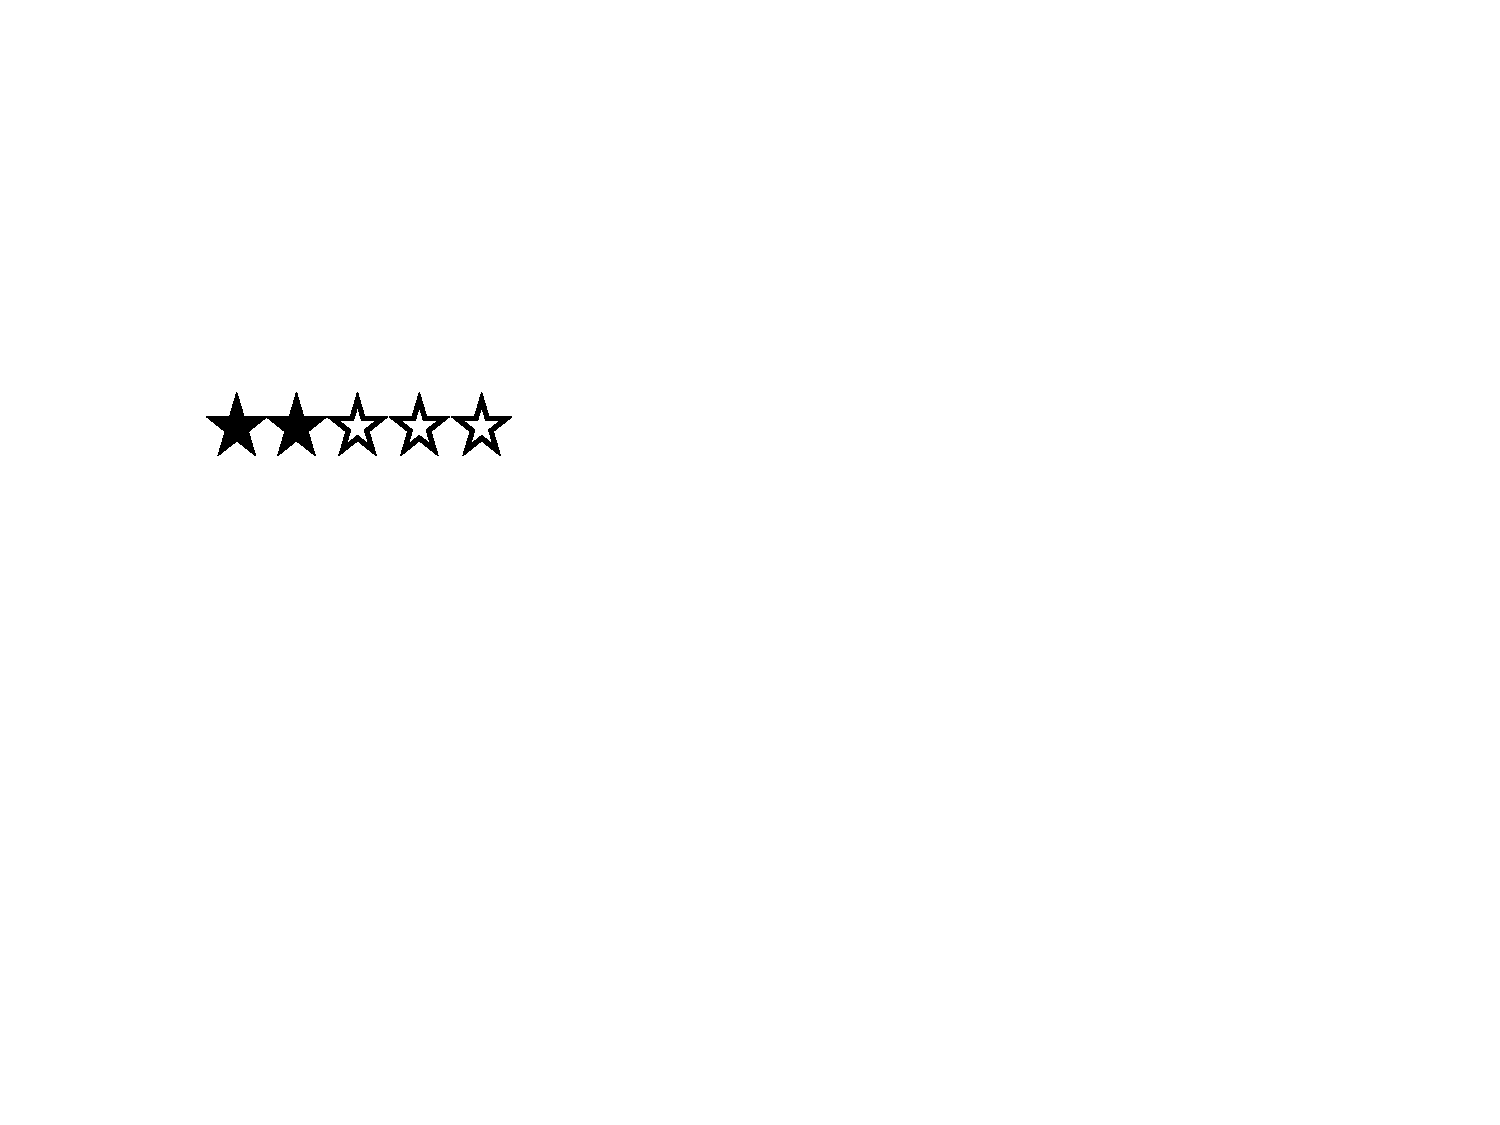
\includegraphics[height=9px]{images/two-stars.pdf}}			&  6 	    	\\
    \hline
    P4				& Software Developer     			& \raisebox{-0.9ex}{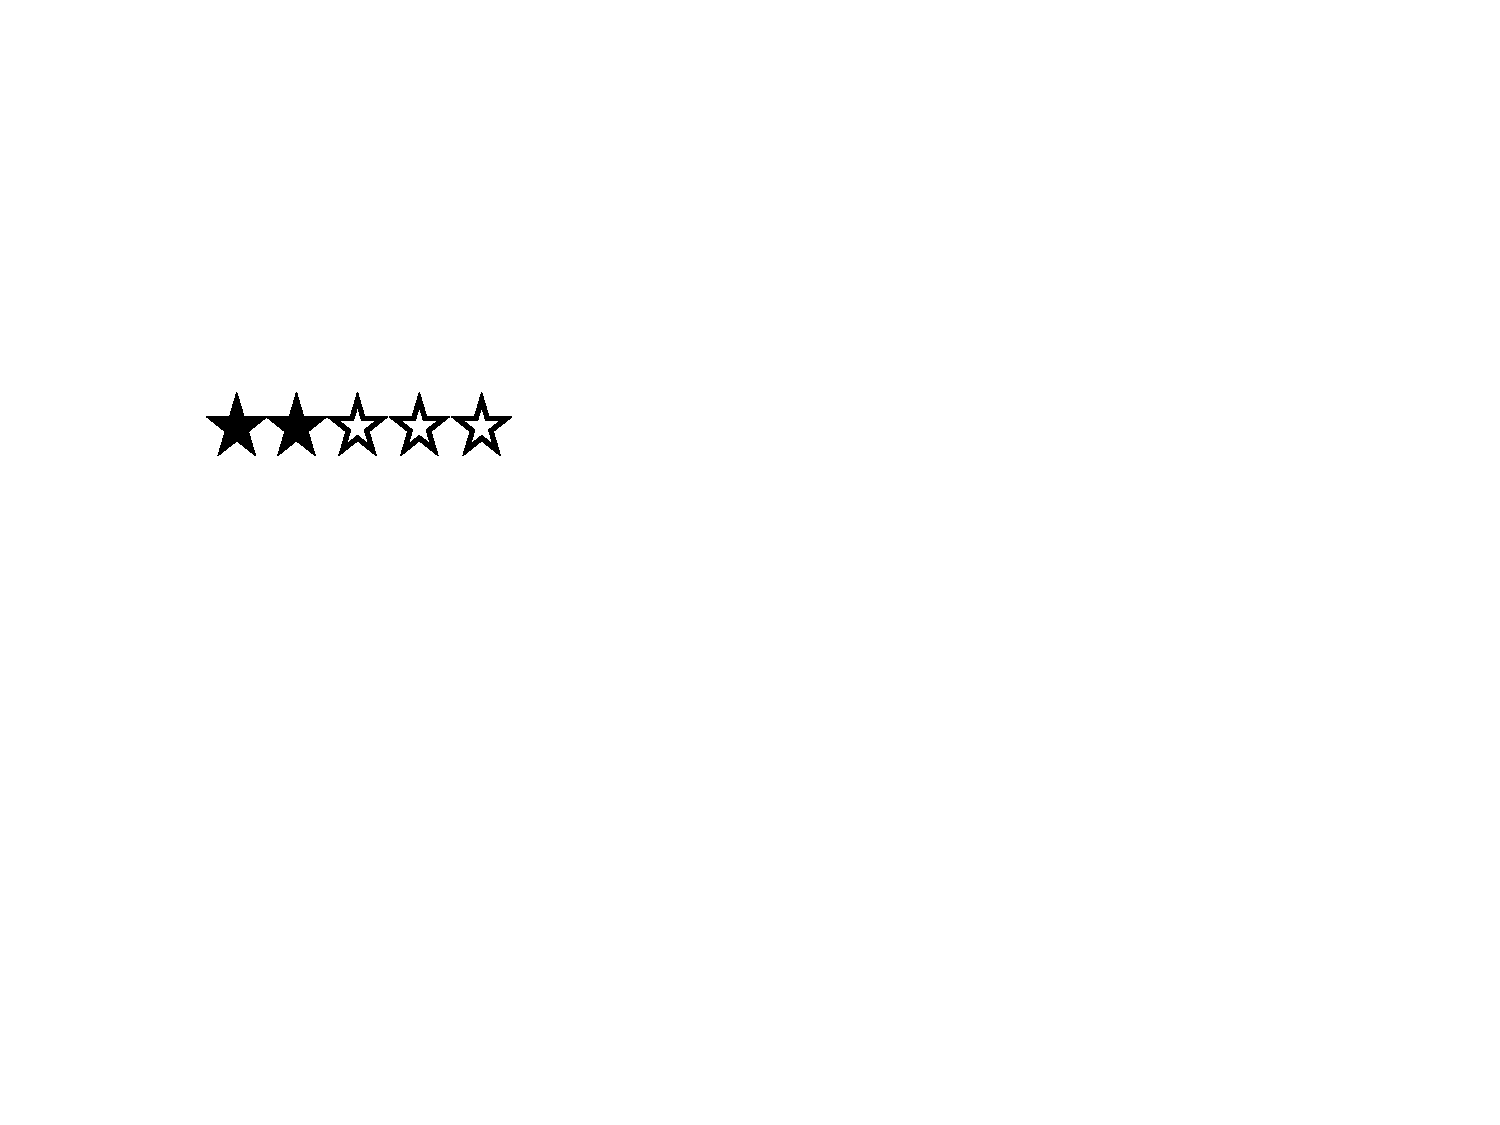
\includegraphics[height=9px]{images/two-stars.pdf}}			&  6     	\\
    \hline
    P5				& Student      						& \raisebox{-0.9ex}{
\includegraphics[height=9px]{images/four-stars.pdf}}			&  10 	\\
    \hline
    P6				& Student		    				& \raisebox{-0.9ex}{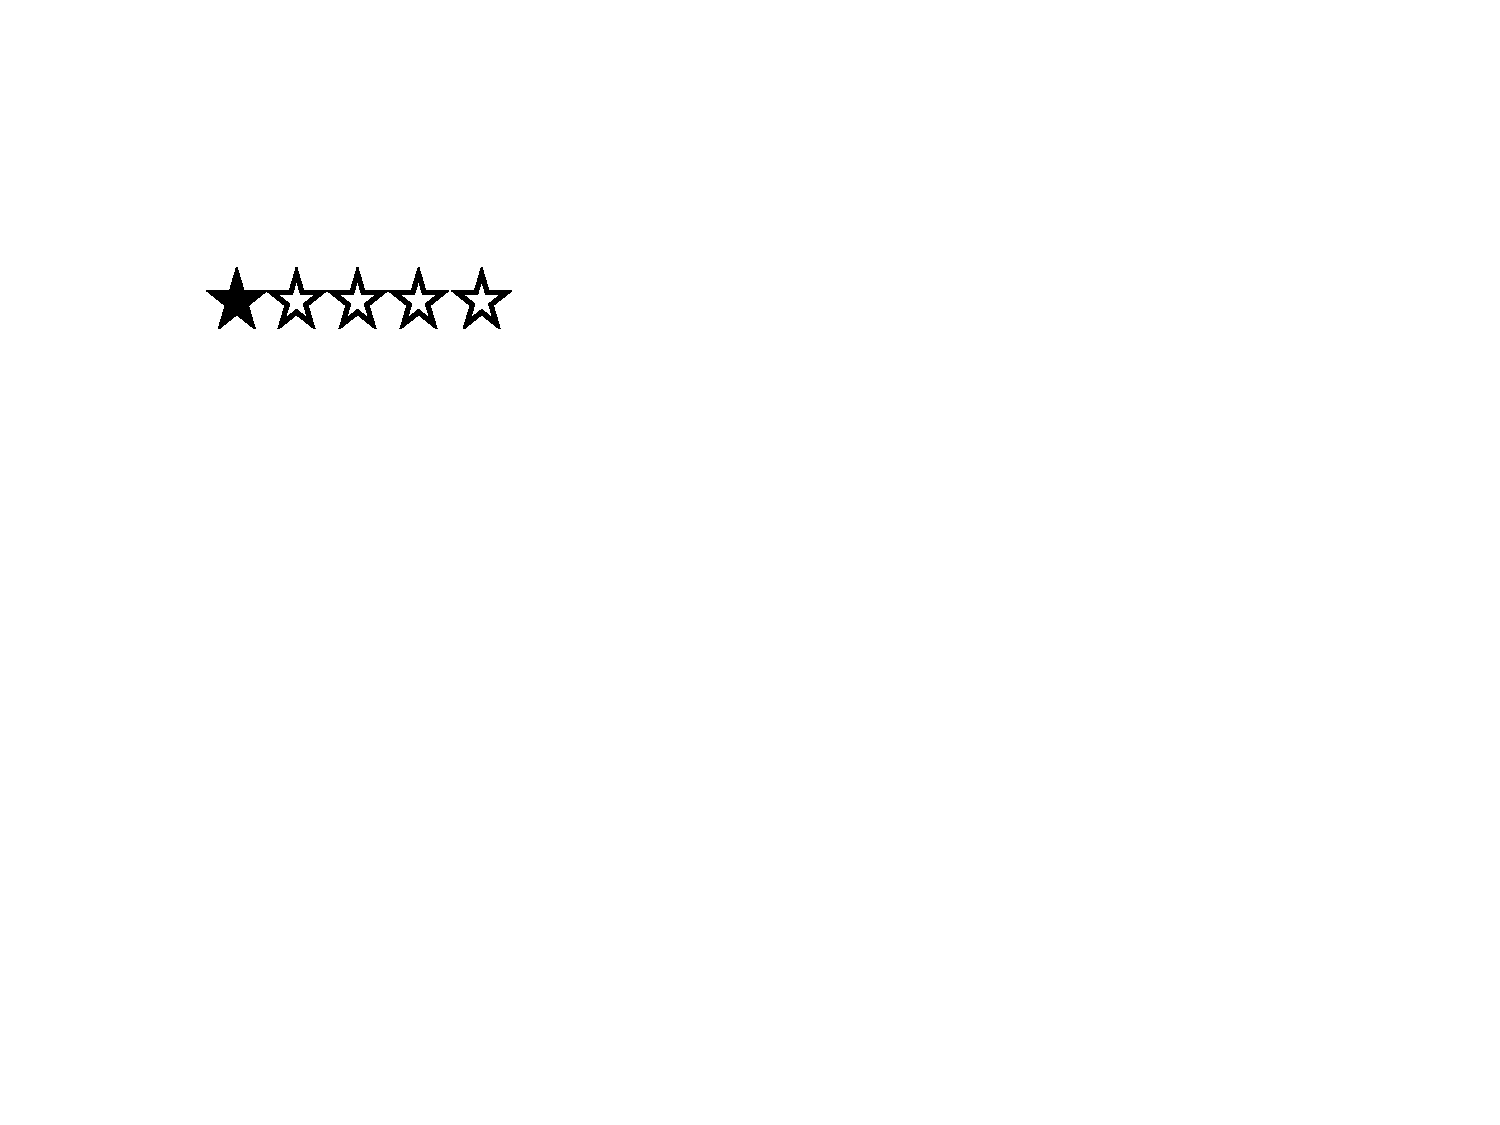
\includegraphics[height=8.5px]{images/one-star.pdf}}				& 4		\\
    \hline
    P7				& Front-end Software Developer    	& \raisebox{-0.9ex}{
\includegraphics[height=9px]{images/four-stars.pdf}}		& 4.5         \\
    \hline
    P8				& Student	    					& \raisebox{-0.9ex}{
\includegraphics[height=9px]{images/three-stars.pdf}}		& 7   \\
    \hline
    P9				& Software Consultant   	 		& \raisebox{-0.9ex}{
\includegraphics[height=9px]{images/three-stars.pdf}}		& 5	  		 \\
    \hline
    P10			    & Student    						& \raisebox{-0.9ex}{
\includegraphics[height=9px]{images/three-stars.pdf}}		& 8	           \\
    \hline
\end{tabular}
\label{table:participants}
\end{table*}



\subsubsection{Participants}

To simulate a more realistic work environment, participants were required to have significant experience working on the iTrust code base. 
All participants either completed or served as teaching assistants for a semester-long software engineering course that focused on developing iTrust.

For our experiment, we recruited 10 software developers, 6 students and 4 professionals. Participants ranged in experience from 4 to 10 years, averaging 6.3 years.
All interviews were conducted in-person.
We recruited participants from personal contacts and class rosters, using snowball sampling to find additional qualified participants.
Since extracting data from each interview required intensive analysis, we ceased recruitment when we felt that we had reached saturation and few new questions were emerging from each additional interview.

Table~\ref{table:participants} gives additional demographic information on each of the 10 participants. 
Since the focus of our study was to identify the questions developers ask independent of their background, we report on demographic information to ensure a degree of diversity in our sample and contextualize participants' responses.

\subsubsection{Tasks}
Each participant was asked to assess four vulnerabilities. 
We presented each participant with this number of vulnerabilities, because in preliminary pilot sessions, participants spent approximately 10-15 minutes with each vulnerability and showed signs of fatigue after 60 minutes.

When selecting tasks, we gave preference to existing iTrust vulnerabilities and sought a broad set of question topics.  
FSB groups similar error messages using a system of topic tags. For example the Null Pointer tag (NP) applies to notifications that warn about the misuse of null. 
To cover a broader set of question topics, we selected vulnerabilities with four different topic tags.
FSB identified three types of naturally occurring vulnerabilities: cross site scripting, path traversal, and predictable random vulnerabilities.
We inserted an SQL injection vulnerability by making minimal alterations to one of the database access objects.
Our modification preserved the functionality of the original code and was based on simple, toy examples of SQL injection presented by OWASP.
Table \ref{table:vulnerabilities} summarizes each of the four vulnerabilities. 

\begin{table*} 
\centering
\caption{Four vulnerability exploration tasks}
\begin{tabular}{|l|l|l|l|}
\rowcolor{gray!50}
\hline
    Vulnerability				& Short Description													& Tool's Rank 						& Tool's Confidence\\
    \hline	
    Potential Path Traversal	& An instance of java.io.File is created to read a file.     			& ``Scary''							 	&  Normal\\
    \hline
    Predictable Random			& Use of java.util.Random is predictable. 								& ``Scary''								&  Normal\\
    \hline
    Servlet Parameter 			& The method getParameter returns a String value that is controlled by the client.			& ``Troubling''		&  Low\\
    \hline
    SQL Injection				& [Method name] passes a non-constant String to an execute method on an SQL statement.     	& ``Of Concern''		&  Low\\
    \hline
\end{tabular}
\label{table:vulnerabilities}
\end{table*}

During the briefing section, we asked participants to pretend they are in charge of security for iTrust and to approach the vulnerabilities as if they were in their normal work environment.
Additionally, we asked them to use a think-aloud protocol, which encourages the participant to verbally announce their thought process as they complete a task or activity~\cite{nielsen2002getting}. 
Specifically, they were asked to, ``Say any questions or thoughts that cross your mind regardless of how relevant you think they are.''

The session moderator was equipped with the following questions, but had the freedom to omit questions and ask follow-up questions based on the participant's responses.
\begin{itemize}
\item What are you exploring/trying to figure out right now?
\item What information do you need to proceed?
\item Can you explain what this warning is trying to tell you?
\item Based on your understanding of this error message, what is the percentage likelihood you would modify this section of he code?
\item How would you fix the problem? Where would you start?
\item On a scale of 1-5, how confident are you in your understanding of the error message?
\item On a scale of 1-5, how confident are you that you are making the correct judgments?
\item What information would you like to see added to the error message?
\item What part of the message is most helpful?
\item Look at the error message one last time. Is there any information you initially disregarded?
\item Would you like to share any other thoughts about this vulnerability?
\end{itemize}

\subsection{Data Analysis}
\label{dataAnalysis}
We analyzed session data using an approach inspired by grounded theory~\cite{glaser2009discovery}. 
First, we transcribed all the audio-video files using oTranscribe.\footnote{\url{otranscribe.com}}
Each transcript, along with the associated recording, was analyzed by two of the authors for implicit and explicit questions. 
The two question sets for each session were then iteratively compared against each other until the authors reached agreement on the question sets. 
In the remainder of this section, we will detail the question extraction process and question sorting processes, including the criteria used to determine which statements qualified as questions.
\subsubsection{Question Criteria}
Participants ask both explicit and implicit questions. 
Drawing from previous work on utterance interpretation, we developed 5 criteria to assist in the uniform classification of participant statements~\cite{letovsky1987cognitive}. 
A statement was coded as a question only if it met one of the following criteria:

\begin{itemize}
\item \textbf{The participant explicitly asks a question.}
\\ P2: \textit{Why aren't they using Prepared Statements?}
\item \textbf{The participant makes a statement and explores the validity of that statement.}
\\ P6: \textit{It doesn't seem to have shown what I was looking for. Oh, wait! It's right above it...}
\item \textbf{The participant uses key words such as, ``I assume,'' ``I guess,'' or ``I don't know.''}
\\ P8: \textit{I don't know that it's a problem yet.}
\item \textbf{The participant clearly expresses uncertainty over a statement.}
\\ P10: \textit{Well, it's private to this object, right?}
\item \textbf{The participant clearly expresses a knowledge requirement by describing plans to acquire information.}
\\ P1: \textit{I would figure out where it is being called.}

\end{itemize}

\subsubsection{Question Extraction}
Using the criteria outlined in the previous section, two of the authors independently coded each session. 
When we identified a statement that satisfied one or more of the criteria, we marked the transcript, highlighting the participant's original statement, and clarified the question being asked.
From the 10 sessions, the first coder extracted 421 question statements; the other coder extracted 389. 

Since participants used a think-aloud protocol, the transcripts contained many statements that were difficult to classify as questions. 
The criteria help ensure that only the statements that reflected actual questions were classified as such. 
Two independent reviewers coded the transcripts to help identify more of the questions being asked, especially the difficult to interpret questions.

Figure \ref{fig:merging} depicts a section of the questions extracted by both authors from P8 prior to review.
\subsubsection{Question Review}
To remove duplicates and ensure the validity of all the questions, each transcript was reviewed jointly by the two authors that initially coded it.
During the second pass, the two reviewers examined each question statement, discussing the justification for each question based on the previously stated criteria.
The two reviewers merged duplicate questions, favoring the wording that was most strongly grounded in the experiment artifacts.

Each question that was only identified by one author required verification.
If the other author did not agree that such a question met at least one of the criteria, the question was removed from the question set and counted as a disagreement.
The reviewers were said to agree when they merged a duplicate or verified a question.Depending on the participant, inter-reviewer agreement ranged from 91\% to 100\%. Across all participants, agreement averaged to 95\%.
High agreement score indicates that the two reviewers consistently held similar interpretations of the question criteria.


Figure \ref{fig:merging} depicts a section of the questions extracted by both authors from P8 prior to review.

\begin{figure*}
\centering
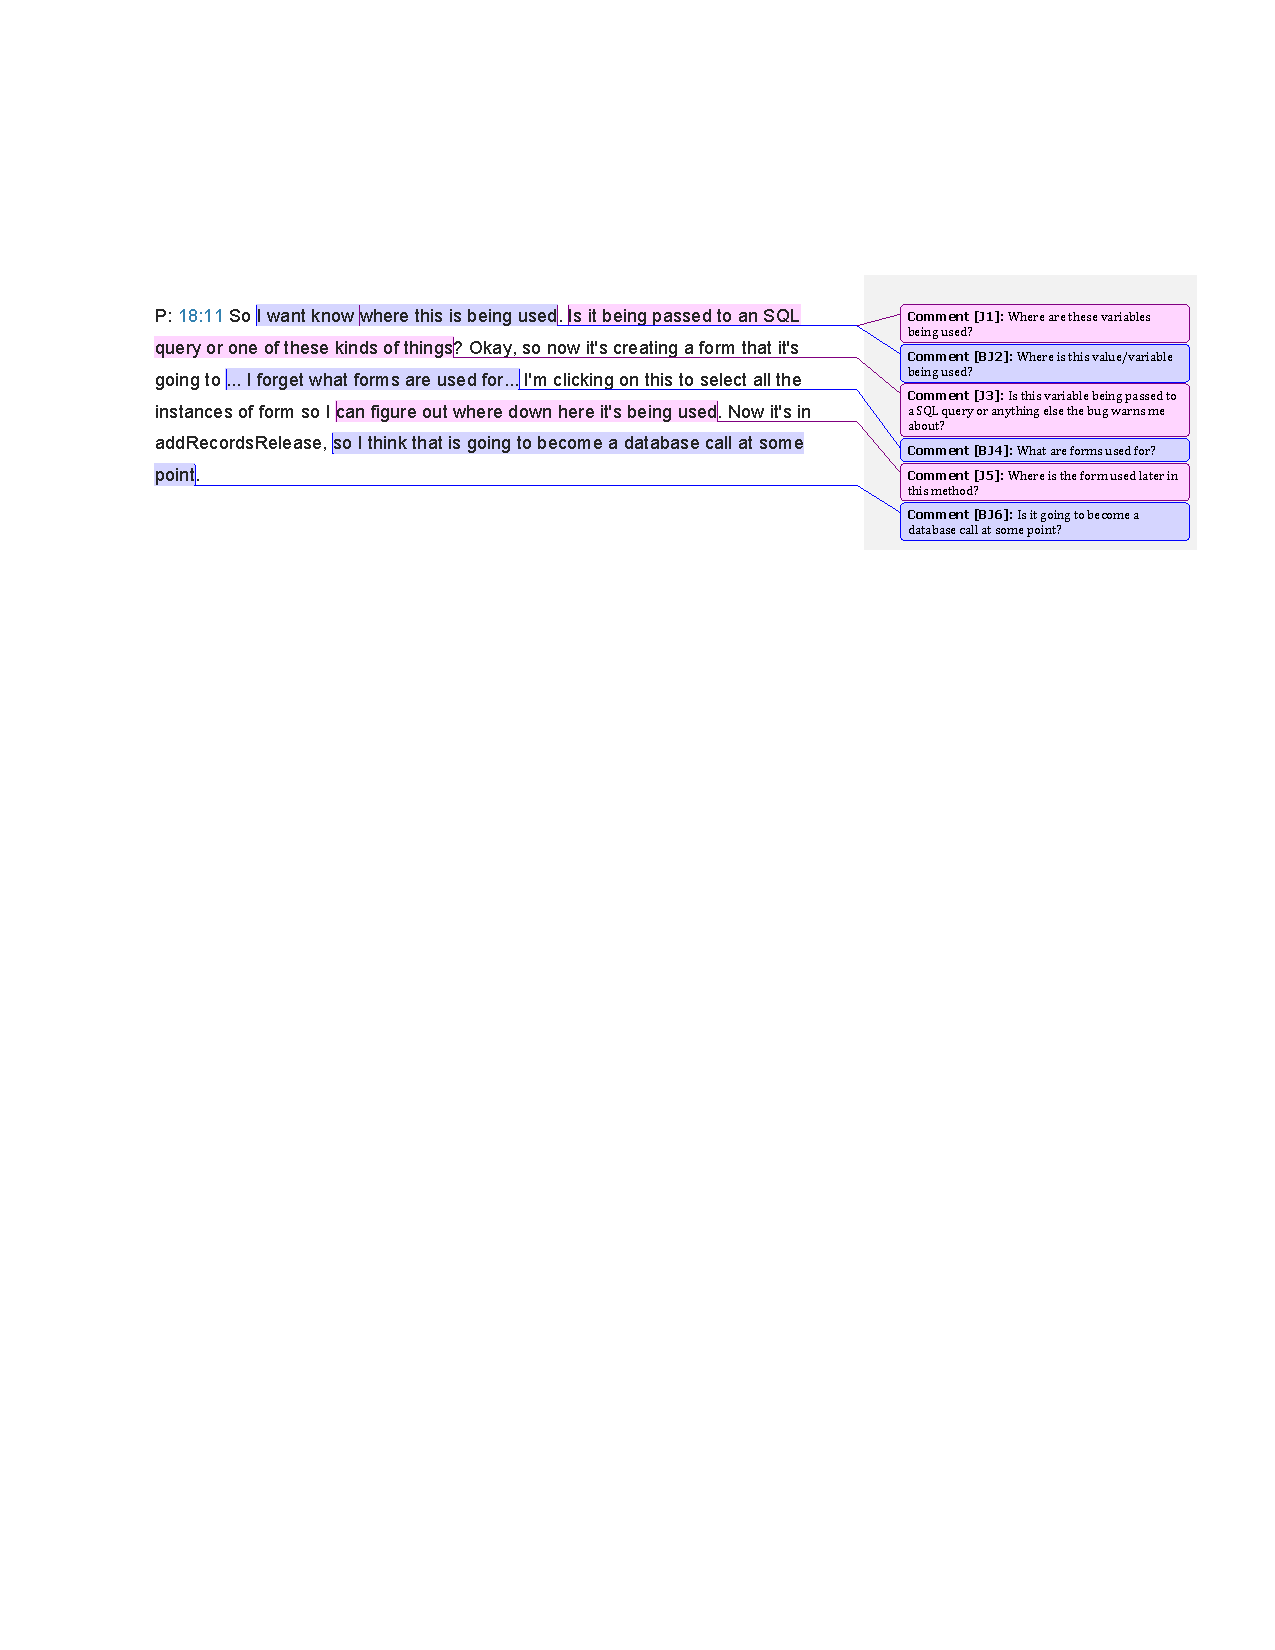
\includegraphics[width=7.5in]{Images/QuestionMerging}
\caption{Question merging process}
\label{fig:merging} 
\end{figure*}

\subsubsection{Question Sorting}
To organize our questions and facilitate discussion, we performed an \textit{open} card sort~\cite{hudson2013sorting}. 
Card sorting is typically used to help structure data by grouping related information into categories. 
In an \textit{open} sort, the process begins with no notion of predefined categories. 
Rather, sorters derive categories from emergent themes in the cards. 

\begin{figure}
\centering
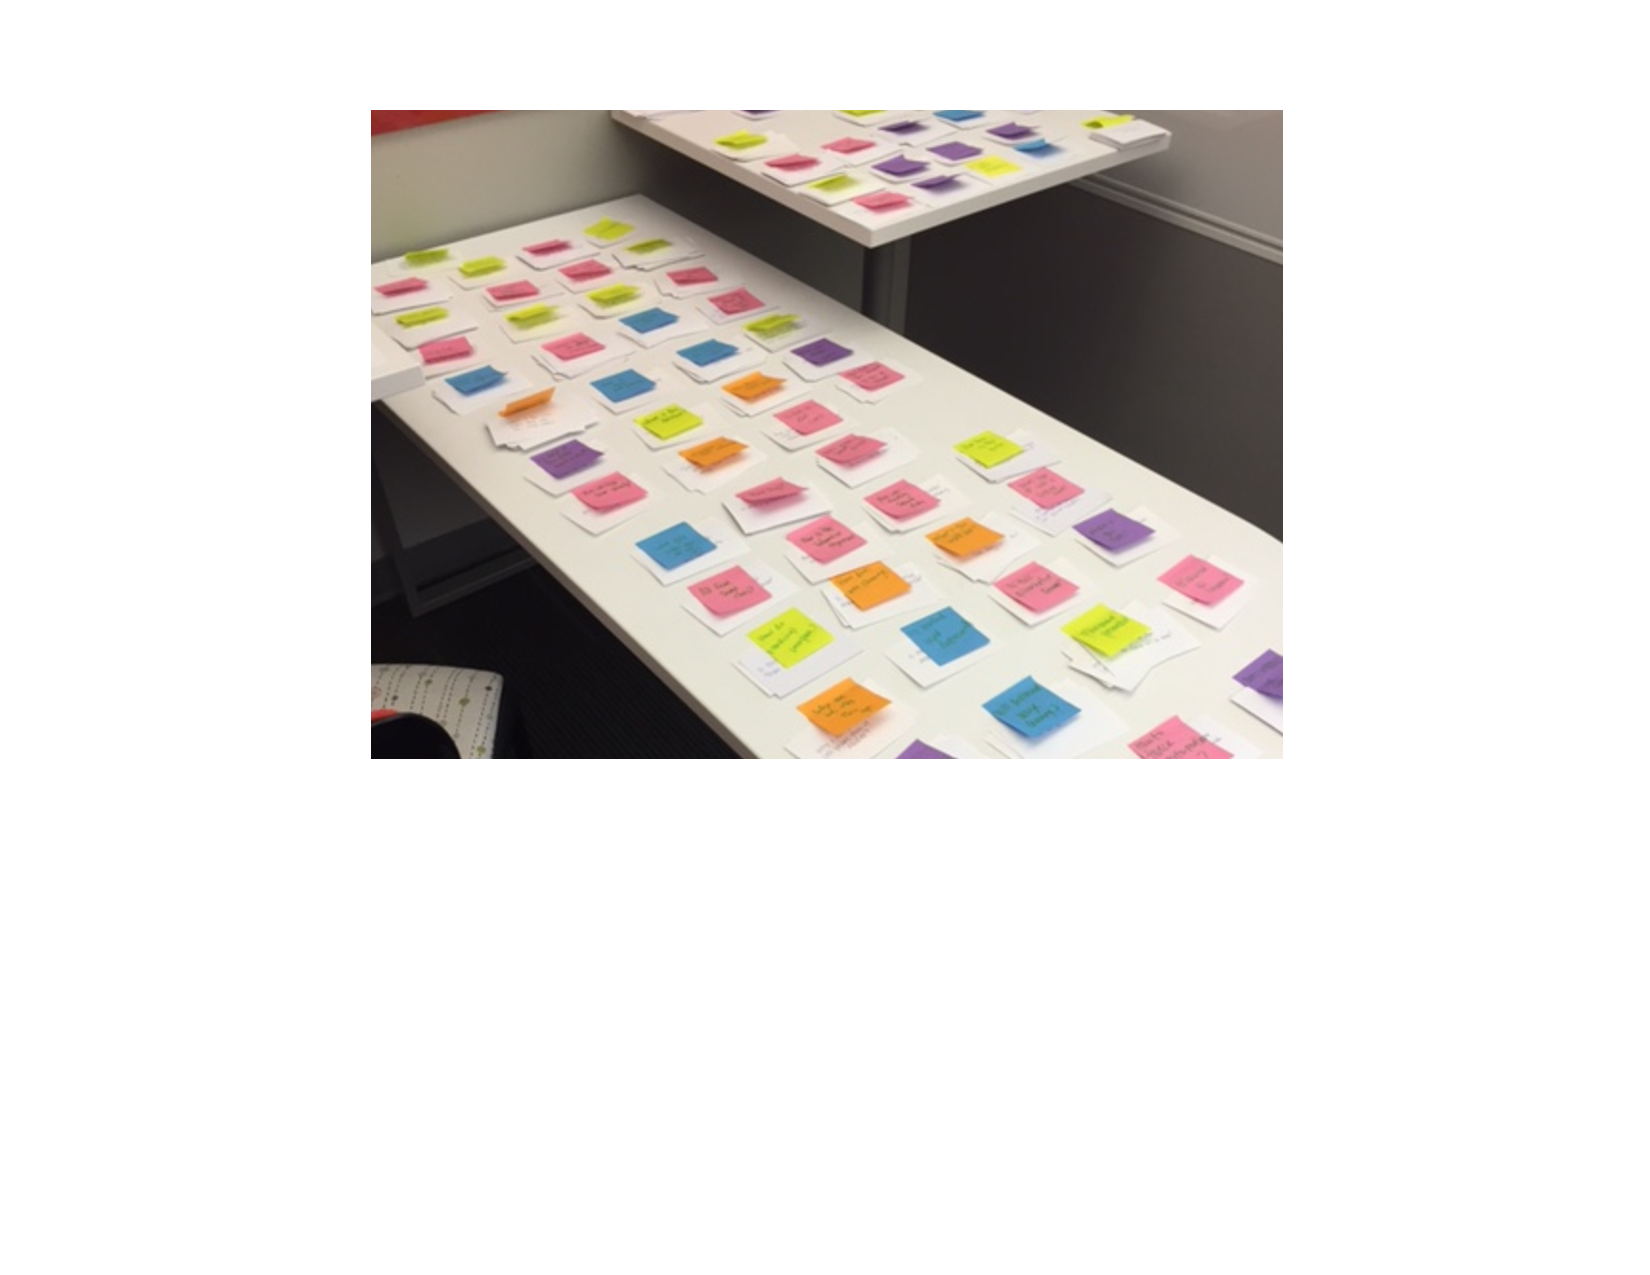
\includegraphics[width=3in]{Images/notecards.pdf}
\caption{Result of phase one of card sorting.}
\label{fig:stageOne} 
\end{figure}

We performed our card sort in three distinct stages: clustering, categorization, and validation.
 
In the first stage, we formed question clusters by grouping questions that identified the same information requirements (Figure~\ref{fig:stageOne}). 
In this phase we focused on phrasing similar questions consistently and grouping duplicates.
For example, P1 asked, \textit{Where can I find information related to this vulnerability?} P7 asked, \textit{Where can I find an example of using prepared statements?} and P2 asked, \textit{Where can I get more information on path traversal?} 
Of these questions, we created a question cluster labeled \textit{Where can I get more information?}
At this stage, we discarded 5 unclear or non pertinent questions and organized the remaining 554 into 155 unique question clusters.

\begin{figure}
\centering
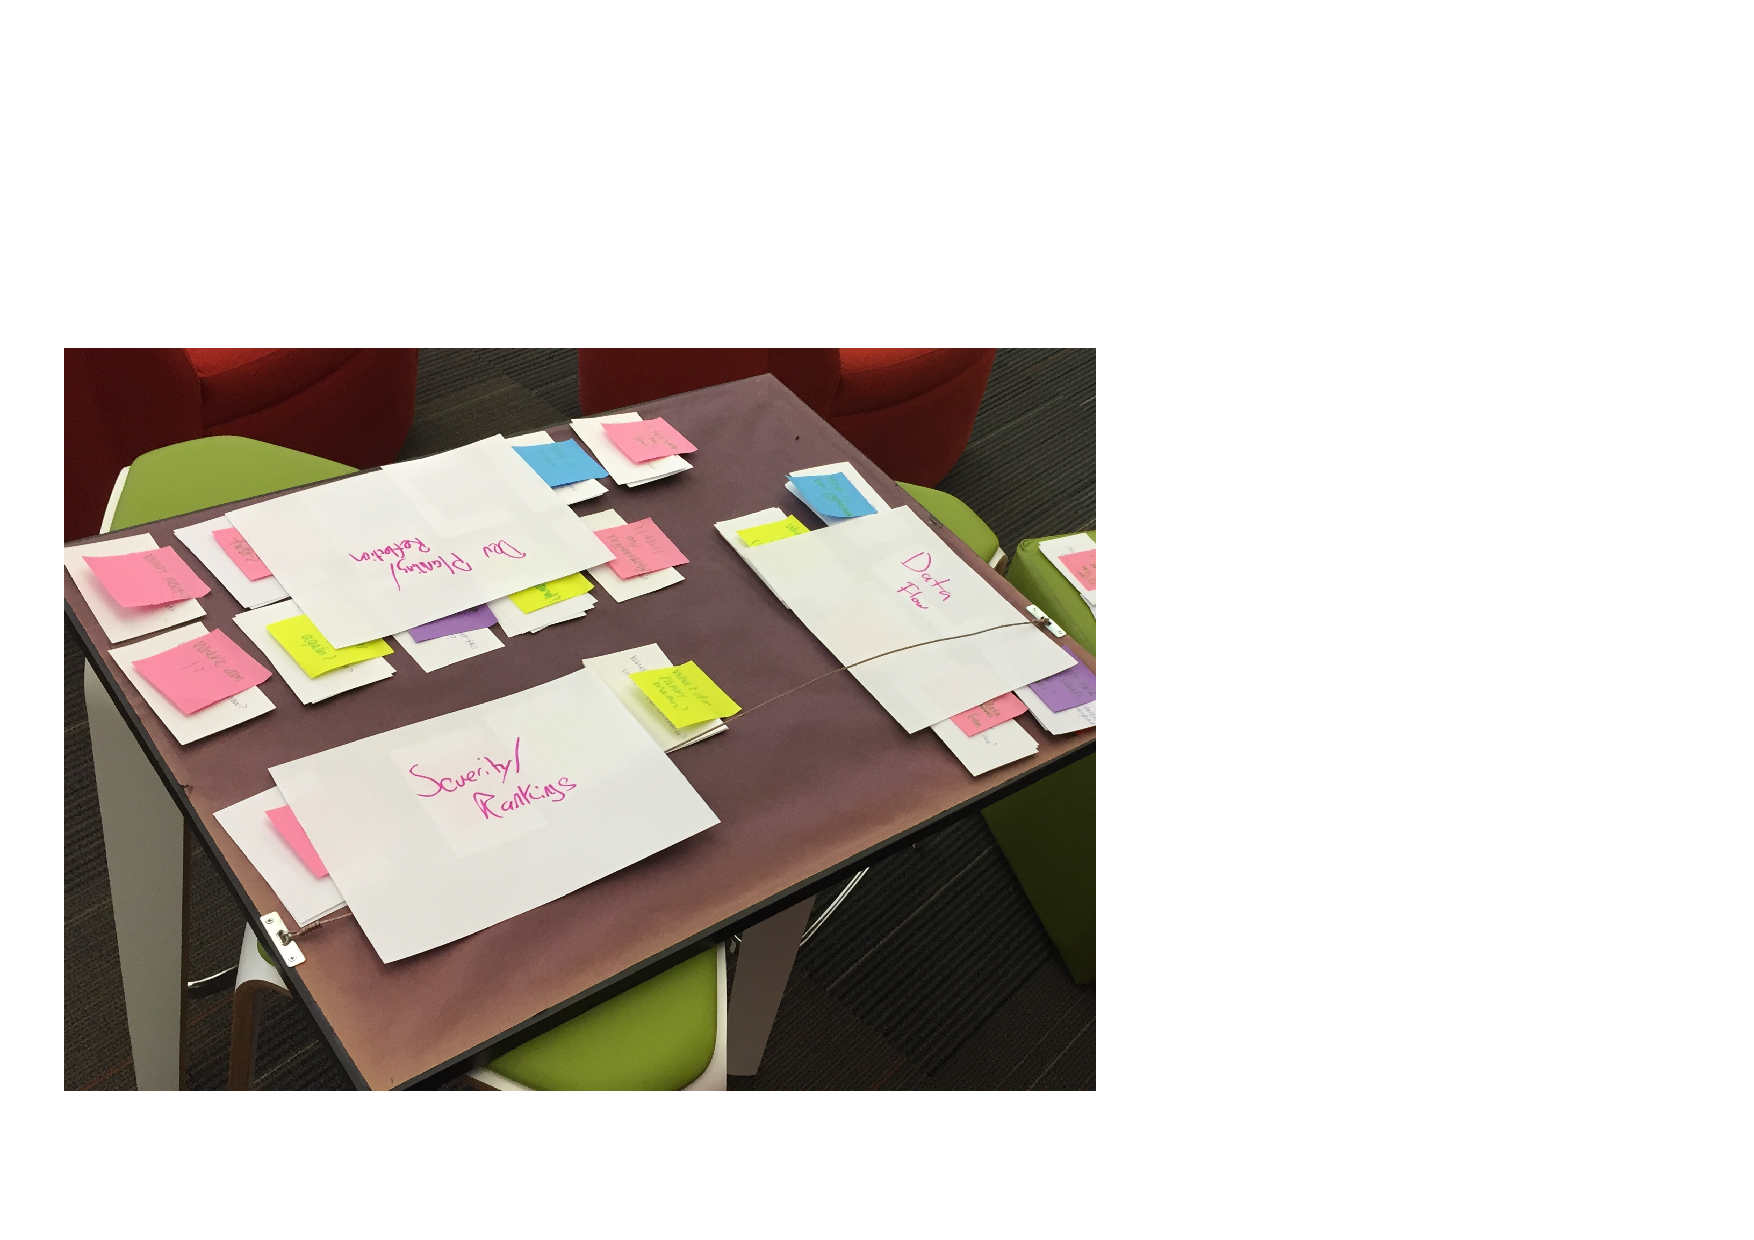
\includegraphics[width=3in]{Images/categories.pdf}
\caption{Sorting cards into categories based on emergent themes.}
\label{fig:cardsort} 
\end{figure}


\begin{table*} 
\centering
\caption{Emergent categories from card sort}
\begin{tabular}{|l|c|c|l|}
\rowcolor{gray!50}
\hline
    Category											& Count		& Location in Paper			& Example 	\\
    \hline		
    Code Background and Functionality	 				& 17     	& Section~\ref{cbf}				& \emph{Example question...}			\\
    \hline
    Developer Planning and Self-Reflection				& 14    	& Section~\ref{dpr}				& \emph{Example question...}			\\
    \hline
    Control Flow and Call Information					& 13     	& Section~\ref{cf}				& \emph{Example question...}		\\
    \hline
    Data Storage and Flow								& 11     	& Section~\ref{dsf}				& \emph{Example question...}		\\
    \hline
    Understanding Alternative Fixes and Approaches		& 11     	& Section~\ref{uafa}			& \emph{Example question...}			\\
    \hline
    Locating Information 								& 11      	& Section~\ref{li}				& \emph{Example question...}			\\
    \hline
    Preventing and Understanding Potential Attacks		& 11     	& Section~\ref{pupa}			& \emph{Example question...}			\\
    \hline
    Resources and Documentation							& 10     	& Section~\ref{rd}				& \emph{Example question...}			\\
    \hline    
    Application Context/Usage							& 9     	& Section~\ref{acu}				& \emph{Example question...}			\\
    \hline
    Understanding and Interacting with Tools			& 9     	& Section~\ref{uit}				& \emph{Example question...}			\\
    \hline
    Assessing the Application of the Fix				& 9     	& Section~\ref{aaf}				& \emph{Example question...}			\\
    \hline
    Understanding Concepts								& 6 		& Section~\ref{uc}				& \emph{Example question...}				\\
    \hline
    Bug Severity and Rank								& 4     	& Section~\ref{bsr}				& \emph{Example question...}			\\
    \hline
    Relationship Between Bugs							& 3     	& Section~\ref{rbb}				& \emph{Example question...}			\\
    \hline
    End-User Interaction								& 3     	& Section~\ref{eui}				& \emph{Example question...}		\\
    \hline
    Error Messages										& 3     	& Section~\ref{em}				& \emph{Example question...}			\\
    \hline
    Confirming Expectations					 			& 1			& Section~\ref{ce}				& \emph{Example question...}   \\
    \hline
    Uncategorized										& 10    	&						& \emph{} \\
    \hline
\end{tabular}
\label{table:categories}
\end{table*}


In the second stage, we identified emergent themes and grouped the clusters into categories based on the themes. 
For example, we placed the question \textit{Where can I get more information?} into a category called \emph{\textbf{Resources/Documentation}}, along with questions like \textit{Is this a reliable/trusted resource?} and \textit{What information is in the documentation?} 
Table~\ref{table:categories} contains the 17 categories along with the number of distinct clusters each contains. 

To validate the categories that we identified, we asked two independent researchers to sort the question clusters into our categories. 
Rather than sort the entire set of questions, we randomly selected 43 questions for each rater to sort.
The first rater agreed with our categorization with a Cohen's Kappa of $\kappa = .63$. 
Between the first and second rater we reworded and clarified some ambiguous questions. The second rater exhibited greater agreement ($\kappa = .70$). 
These values are within the $.60 - .80$ range, indicating substantial agreement~\cite{Landis1977agreement}.

\section{Results: Vulnerabilities, Attacks, and Fixes, Oh My!}
\label{sec:results-vaf}
We list each distinct question we extracted and the count for each in parentheses. For each category, we discuss the common thread that ties questions in that category together. 
We also contextualize each category by discussing existing tool support and shortcomings.
Categories have been places into four groups to facilitate discussion: Vulnerabilities, Attacks, and Fixes, Oh My!; Code and the Application; Individuals; and Problem Solving Support.
% next paragraph, go into description of first group 


%%%%%%%%%%%% Understanding Alt. Fixes

\noindent\subsection{\textbf{Understanding Alternative Fixes and Approaches (8)}}\label{uafa}

When resolving security vulnerabilities, participants encountered alternative approaches that appeared to achieve the desired functionality more securely.
For example, when evaluating the SQL injection vulnerability, participants found resources that suggested using the Prepared Statement Class instead of Java Statements. 
Participants found many sources for alternative fixes, including web resources and even code located in other parts of the project.
When presented with alternative approaches, participants compared the alternative with the current code and assessed the applicability of the alternative. 
Eleven of the 155 questions we extracted pertained to understanding the various facets of alternative approaches or solutions, such as:
\\
\\
\noindent\emph{Does the alternative function the same as what I'm currently using? (6)} \\
\emph{What are the alternatives for fixing this? (4)} \\
\emph{Are there other considerations to make when using the alternative(s)? (3)} \\
\emph{How does my code compare to the alternative code in the example I found? (2)}
\emph{Why should I use this alternative method/approach to fix the vulnerability? (2)} \\
\emph{When should I use the alternative? (1)} \\
\emph{Is the alternative slower? (1)} \\

\noindent\textbf{Observations}
%The developer could attempt to apply the new fix or approach, but the data we report in Section~\ref{aaf} suggests developers also have questions about this process that make it difficult to quickly and effectively complete.
%SAVE THIS CONNECTION FOR LATER
Eight participants had questions that fit into this category. 
The FSB notifications for the SQL Injection and Predictable Random vulnerabilities explicitly offer alternative fixes. 
As noted, the message associated with the SQL Injection vulnerability suggests switching to use Prepared Statements. 
The message associated with the Predictable Random vulnerability suggests switching to use \textit{java.security.secureRandom}. 
In other cases, participants turned to a variety of sources, such as StackOverflow, official documentation, and personal blogs for alternative approaches. 
Three participants specifically mentioned StackOverflow as a source for better understanding alternative approaches and fixes. 
P7 preferred StackOverflow as a resource, because it included real-world examples and elaborated on what was wrong with the code as it was currently written.  
While attempting to assess the Servlet Parameter vulnerability (Table~\ref{table:vulnerabilities}), P8 decided to explore some resources on the web and came across a resource that appeared to be affiliated with OWASP.~\footnote{\url{https://www.owasp.org/index.php/Main_Page}} 
Because he recognized OWASP as ``the authority on security,'' he clicked the link and used it to make is final decision regarding the vulnerability. 
Despite the useful information that some participants found, often the candidate alternative did not readily provide meta-information about trade-offs or the process of applying suggestions. 
For example, P9 found a suggestion on StackOverflow that he thought might work, but it was not clear if it could be applied to the code in iTrust. 
\\

\noindent\textbf{Tool Implications} 
It seems especially important when dealing with potential security vulnerabilities that developers fully understand any changes they make to the code. 
However, based on our observations, developers lack easy-access to security-relevant information on potential alternatives. 
Rather, participants used ad-hoc strategies to seek different pieces of information from a variety of sources. 

The questions in this category suggest that developers could use a tool that aggregates information on alternative secure coding practices.
Our observations also suggest that such a tool should include real world examples and draw from trusted authorities on security.
Finally, the tool should present information about the trade-offs associated with a particular alternative, such as decreased performance or the possibility of introducing additional vulnerabilities. 

%One way a tool might help developers determine the changes, if any, they should making would be by noting other places in the code the alternative under  consideration has been used, if they exist. 

%The tool could then potentially use speculative analysis, which is used by tools like \textsc{Quick Fix Scout}, to present trade-offs of using the suggested fix or keeping the code as it is~\cite{mucslu2012speculative}.

%GOOD POINTS ABOVE NOT SURE HOW THEY FIT WITH STORY


%If the developer, or other developers of the code, have not used the alternative before, the tool could borrow behavior or design principles from \textsc{Whyline} by allowing developers to ask questions about the code in relation to the suggested approach~\cite{ko2004designing}. 



%%%%%%%%%%%% Preventing and Understanding Potential Attacks 

\noindent\subsection{\textbf{Preventing and Understanding Potential Attacks (10)}}\label{pupa}
Unlike other types of code defects that may cause code to function unexpectedly or incorrectly, security vulnerabilities open the code up to potential attacks. For example, the servlet parameter vulnerability introduced the possibility of SQL injection, path traversal, command injection, and cross-site scripting attacks.
Eleven of the 155 distinct questions we gathered belong in this category.
\\

\noindent\emph{Is this a real vulnerability? (7)} \\
\emph{What are the possible attacks that could occur? (5)} \\
\emph{Why is this a vulnerability? (3)} \\
\emph{How can I prevent this attack? (3)} \\
\emph{How can I replicate an attack to exploit this vulnerability? (2)} \\
\emph{What is the problem (potential attack)? (2)} \\
\emph{How can this vulnerability lead to an attack? (1)} \\
\emph{How should I address this problem? (1)} \\
\emph{How do I find out if this is a real vulnerability?(1)} \\

\noindent\textbf{Observations}
Participants sought general information relating to the attacks in a given context.
To that end, five participants asked \textit{What are the possible attacks that could occur?}
For example, within the first minute of his analysis, P2 stated that he was thinking about the different types of attacks that could target web applications, like iTrust.

On the other hand, participants also sought specific attack-information regarding the vulnerability at hand.
Participants hypothesized about specific attack vectors, how to execute those attacks, and how to prevent those attacks now and in the future.
Seven participants asked the question, \textit{Is this a real vulnerability?} To answer that question, participants searched for hints that an attacker could actually execute an attack in the given context. For example, P10 determined that the Predictable Random vulnerability was ``real,'' because an attacker could deduce the random seed and use that information to determine other users' passwords. 
\\

\noindent\textbf{Tool Implications}
Unlike other contexts, when analyzing security vulnerabilities, developers ask questions pertaining to potential attacks.
Trivially, the existence of this category suggests that security tools should be designed differently from other code analysis tools; they should present pertinent information about potential attacks attacks.

However, the questions in this category also suggest that developers operate in two distinct modes when reasoning about potential attacks.
At times they inquire about all the possible attacks that could occur.
At other times, they explore the feasibility of a specific attack.
Security tools should support this modality by separating information about all the possible attacks from more detailed information about specific attacks.

%Some Find Security Bugs notifications attempt to provide developers with the means to answer some of these questions by providing links to relevant information. 
%Many of the links provided linked to information regarding why the code may be broken, however, do not provide information to improve understanding of what the potential attacks are. 
%Some of the questions, such as \textit{How do I find out if this is a real vulnerability?}, may not be as simple to answer by providing a link. 
%This kind of question may require triangulation of information; some information from the web on the vulnerability itself and the potential attacks, and some information from fellow developers who may better understand the likelihood the bug is a vulnerability in their system. 
%One way tools can help is by providing easy access to the top web resources and developers to use when assessing the vulnerability; many of our participants preferred StackOverflow as a resource and a degree of knowledge model, like the one proposed by Fritz and his colleagues, could provide the developers most familiar with the code~\cite{fritz2010degree}.


%%%%%%%%%%%% Assessing Application % % % % % % % % % % % % % % % % % % % % % % % %

\noindent\subsection{\textbf{Assessing the Application of the Fix (9)}}\label{aaf}
Once participants had identified a specific approach for fixing a security vulnerability, they asked questions about applying the fix to the code.
For example, when considering the use of \textit{java.security.secureRandom} to resolve the Predictable Random vulnerability, participants questioned the applicability of the fix and consequences of making the change. 
The questions in this category differ from those in \emph{\textbf{Understanding Alternative Fixes and Approaches}} (Section \ref{uafa}); 
These questions focus on the process of applying  and reasoning about a given fix, rather than identifying and understanding possible fixes.
We placed 9 of the 155 distinct questions into this category.
\\

\noindent\emph{Will the error go away when I apply this fix? (5)} \\
\emph{How do I use this fix in my code? (4)} \\
\emph{How do I fix this vulnerability? (4)} \\
\emph{How hard is it to apply a fix to this code? (3)} \\
\emph{Is there a quick fix for automatically applying a fix? (2)} \\
\emph{Will the code work the same after I apply the fix? (2)} \\
\emph{What other changes do I need to make to apply this fix? (2)} \\
\emph{Can these fix suggestions be applied to my code? (1)} \\
\emph{Does the code stand up to additional tests prior to/after applying the fix? (1)} \\


\noindent\textbf{Observations}

When searching for approaches to resolve vulnerabilities, participants gravitated toward quick fixes.
The notifications associated with the Predictable Random vulnerability and the SQL Injection vulnerability both provided quick fix suggestions.
All participants proposed solutions that involved applying one or both of these quick fixes. 
Additionally, two participants explicitly asked if quick fixes were available and P2 even commented that it would be nice if all the notifications contained quick fixes.
However, unless prompted, none of the participants commented on the disadvantages of using proposed quick fixes, such as reduced performance or the possibility of introducing another defect.
 
P9 had a noteworthy experience while exploring the Predictable Random vulnerability. Unlike the other participants, he missed the part of the error message that described the ``quick fix.'' 
He went on to detail his plans for searching the web for standard random number generation techniques. 
Then he recalled a technique that he had encountered before and explained that he might implement his own random hashing algorithm, but concluded that he would do more searching to find out the best way to apply that fix.
Before proceeding to the next vulnerability, P9 reread the error message, noticed the quick fix and decided he would apply the quick fix instead.
\\

%How hard is it to fix, if fix is easy, then just apply the fix. Don't investegate the consequences. Validate the fix by seeing if the bug icon went away
%without tests or sufficient review to validate the correctness of the fix, such impulsive modifications could have unintended consequences.

\noindent\textbf{Tool Implications}
Assuring the security of complex software systems requires developers to reason critically about the code. 
Quick fixes help developers dismiss vulnerabilities more quickly.
However, especially in security, quicker might not always be better. 
In the case of P9, without the quick fix he searched the web for best-practices and drew conclusions from a broader set of resources.
In some sense, his experience lead him to a better understanding of the vulnerability than those who read the entire notification.
Our observations suggest that the presence of quick fixes alone may discourage developers from fully considering the implications of their proposed changes.

%False positives
Existing tools, such as Quick Fix Scout begin to address this problem by describing what might happen if a quick fix is implemented~\cite{mucslu2012speculative}. 
Quick Fix Scout helps developers consider the implications of implementing a fix.
Security tools that include quick fixes should also encourage developers to assess alternative fixes or whether they need to modify the code at all.
%Though it is not clear how feasible it is to answer some of these questions, some can be answered by using a similar approach to that used by Mu{\c{s}}lu and colleagues when developing 
%Their tool attempts to help developers answer the question \textit{Does this fix introduce other bugs?} 
%None of our participants asked this question specifically, but to that effect, P1 and P2 asked \textit{Will the code work the same after I apply the fix?} 
%Further, questions like \textit{How hard is it to apply?} and \textit{Does the code stand up to additional tests prior to/after applying the fix?} could possibly be answered using a similar process.


%%%%%%%%%%%% Relationship Between Bugs

\noindent\subsection{\textbf{Relationship Between Bugs (4)}}\label{rbb}

Some participants asked questions about the connections between co-occurring vulnerabilities and whether or not similar vulnerabilities exist elsewhere in the code. 
For example, when participants reached the third and fourth vulnerabilities, they began noticing and speculating about the similarities between the vulnerabilities they inspected.
Three of the 155 distinct questions we found target the relationships between the vulnerabilities in the code. 
\\

\noindent\emph{Are all the bugs related in my code? (3)} \\
\emph{Does this other piece code have the same bug as the code I'm working with? (1)} \\
\emph{Are all of these notifications vulnerabilities? (1)} \\


\noindent\textbf{Observations}
%P1 2 8 10 asked
%Are all of the bugs related in my code?

When inspecting the Servlet Parameter vulnerability, P8 wondered if other parts of the code contained similar vulnerabilities.
NOT MUCH TO SAY HERE?

\noindent\textbf{Tool Implications}

%Make more clear, This is the implication, but doesn't jump off the page yet...
Though only four of the ten participants asked questions about the relationship between bugs, these questions highlight information requirements that tools could support.
When inquiring about the relationships between bugs, participants noted connections between bugs that related to similar topics.
FSB organized the vulnerabilities it identified based on their locations in the code, or alternatively based on their seriousness.
Grouping vulnerabilities based on abstract concepts might enable developers to focus on areas in which they have expertise, or identify and resolve similar bugs more quickly.

HELP: I know about CWE are there other canonical taxonomies? More importantly, do tools present bugs according to these taxonomies (group based on similar topic)?
%We speculate that developers might have these kinds of questions because they want to know if a vulnerability like the one they are assessing exists in other similar code fragments.
%Another reason for asking this kind of question is to determine the possibility of eliminating more than one vulnerability with one fix. 
%Whatever the motivation may be, participants did not seem to have an intuitive or easy way of going about finding the answer to the questions asked in this category.
%A tool that answers these questions might make visible the connections between the bugs reported, either visually or by augmenting notifications with information regarding this bug's relevance to others in the code.

%Alert prioritization. Particpants ask if notifications in the same area are the same. Research suggests that homogenous errors occur close to one another. Tools should help synthesize these similar notifications to present information to developers more effectively.


\section{Results: Code and the Application}
\label{sec:results-ca}

% description of what categories fall into this group



%%%%%%%%%%%% Locating Information

\noindent\subsection{\textbf{Locating Information (10)}}\label{li}

Some participants asked questions regarding locating, or the ability to locate, information in their coding environment. 
Eleven questions of the 155 extracted fit into this category.
The distinction between this category and \emph{\textbf{Code Background and Function}} is that this category includes questions pertaining to searches made in the coding environment for information, artifacts or code fragments. 
On the other hand, \emph{\textbf{Code Background and Function}} pertains to understanding the code at a higher level that would not be answered by triaging the code.
\\

\noindent\emph{Where is this used in the code? (10)} \\
\emph{Where are other similar pieces of code? (4)} \\
\emph{How do I track this information in the code? (2)} \\
\emph{Where is this artifact? (1)} \\
\emph{Is this artifact located in this class? (1)} \\
\emph{Where is this method defined? (1)} \\
\emph{Where is this class? (1)} \\
\emph{Where is the next occurrence of this variable? (1)} \\
\emph{How do I navigate to other open files? (1)} \\


\noindent\textbf{Observations.}
All 10 participants found themselves in situations where they wanted to know where the code associated with the potential vulnerability is being used throughout the system. 
This most often occurred while assessing the Predictable Random and Servlet Parameter vulnerability. 
The goal of these questions seemed to involve determining if there is a real vulnerability in the code. 
While assessing the Predictable Random vulnerability, P2 and P10 wanted to know if the code the notification was attached to was only run in test code. 
They were able to use existing tools to find where the code was being used, however, P2 was still could not confirm 100\% that the code is only used in tests. % more detailed strategies?

When attempting to understand the Servlet Parameter vulnerability, participants often wanted to determine where the parameter of interest is being used within the system. 
Some participants, like P1, attempted to gather information using existing tools, such as the code element highlighting offered by Eclipse which shows where a code element is being used locally. 
Others mentioned wanting to know where the parameter is used but did not take steps to actually find out; perhaps other participants encountered a situation similar to P6 where they were uncertain of how to start locating the information.

Four participants wanted to find other parts of the code that used similar code to implement system functionality.
For all of them, this was a manual process involving mostly scrolling through and exploring the code. 
For example, while assessing the SQL Injection vulnerability, P2 and P5 both wanted to know more about how the functionality under investigation is implemented in other parts of the code. 
P2 wanted to know, more specifically, what other parts of the code use Database Access Objects.

% question with no tool support for answering
Two participants had questions concerning the ability to track information while interpreting some of the vulnerabilities. 
To better understand the SQL Injection vulnerability, P9 wanted to find a way to track all the possible inputs, with no success. 
P6 wanted to be able to track all the variables that could be affected by this vulnerability; because no tool support to his knowledge existed to help retrieve the information, he noted he would use pencil and paper to do so. 
Because this is a process that could take some time, P6 explained how he would do it rather than doing it, as many participants did when they had tool support.
\\

\noindent\textbf{Tool Implications.}
The answers to most of these questions can be found using existing tool support found inside the IDE. 
For example, Eclipse has an 'open declaration' tool that can be used to find a method's definition. 
A few of these questions, however, requires significantly more effort on the developer's part to answer, therefore could benefit from tool support. 
For instance, participants who asked \textit{how do I track this information in the code} did not have a tool-supported way to answer this question.
Similar to the suggestion made in Section~\ref{cf}, a tool that can automatically detect when a developer is attempting to track specific information could help by either helping the developer track the information of interest or pointing out a tool that can.
Developers could also benefit from tool support when attempting to find other parts of the code written similarly to the potentially vulnerable code; a tool that supports this process might include references to other parts of the code using similar code elements as part of the vulnerability description.



%%%%%%%%%%%% Control Flow/Call Information

\noindent\subsection{\textbf{Control Flow and Call Information (10)}}\label{cf}

We also extracted questions relating to control flow and calling information. 
Developers seek information information pertaining to the methods that get called, or do not get called, in the code. 
As the name of this category suggests, these questions can generally be answered using a tool for viewing the call hierarchy, when available. 
Thirteen of the 155 distinct questions extracted dealt with acquiring control flow and call information.
\\


\noindent\emph{Where is the method being called? (10)} \\
\emph{How can I get calling information? (7)} \\
\emph{Who can call this? (5)} \\
\emph{Are all calls coming from the same class? (3)} \\
\emph{What gets called when this method gets called? (2)} \\
\emph{What is the call hierarchy? (1)} \\
\emph{What causes this to be called? (1)} \\
\emph{How often is this code called? (1)} \\


\noindent\textbf{Observations.}
% All asked "where is method being called?" at some point --> all bugs at least once but mainly B1
All 10 participants wanted control flow or call information for a method in the code at some point; the question \textit{where is this method being called?} was asked at least once for each vulnerability, but showed up the most while participants attempted to interpret the Potential Path Traversal vulnerability.
Eclipse includes a call hierarchy tool that allows users to easily traverse the calls made to a given method, answering questions such as \textit{where is this being called}. 
While most participants located and employed the call hierarchy tool, some used other more error-prone approaches, such as the 'find references' tool or manual visual inspection. 
For example, P1 and P6 chose to use more light-weight tools, such as inspecting code highlights, rather than navigate to and invoke the call hierarchy tool; P1 was unaware of what the call hierarchy tool was. 
P5 and P9, who also did not seem to be aware of the existence of a call hierarchy tool, considered using find references to get the information they needed.

Along the same lines, when assessing the Potential Path Traversal vulnerability, 5 participants wanted to know who can call that code. 
Tools like the call hierarchy tool can inform developers of who \textit{is} calling the code, however, they do not answer the question who \textit{can} call the code. 
To determine how vulnerable this part of the code was, participants wanted to know if the code in question could be called outside the containing class as well as the system. 
Most of the participants who asked this question concerning the containing class answered the question by checking the visibility of the method (\texttt{public} vs. \texttt{private}). 
Determining if the code can be accessed outside the system, was not something participants interested could easily determine so they did not attempt to.
% name exactly who did what?

% Tools available for this but 7 still had question "how can I get calling information?"
Despite the availability of tools to help retrieve call information, some participants still had difficulty finding answers to their questions; seven even asked the question \textit{how can I get calling information}.
For example, P4 did not have any ideas on how he might find call information for the method containing the Potential Path Traversal vulnerability; after struggling with answering his questions for a while, he finally stumbled upon the call hierarchy tool. 
Even after finding and using the tool, P4 still needed other tools, such as the search tool, to come to the conclusion that it was not a vulnerability he needed to be concerned about.
\\


\noindent\textbf{Tool Implications.}
Even with tools like 'find references' and the call hierarchy view tool, it may be difficult to answer questions like \emph{how can I get calling information} and \emph{who can call this} without having to manually, and mentally, aggregate information gathered from different tools. 
Further, even a combination of these tools are ineffective for someone who is unaware of their existence.
A tool that addresses these types of needs might detect when the developer is looking for call information (for example, using the 'find' tool) and suggest the appropriate tool for finding the information they require. 
To increase visibility of the desired information, the tool might also highlight the relevant method as it appears in the call hierarchy or augment each method with the methods that can call it.

%It is unclear whether the call hierarchy tool is more efficient than tools like 'find references' for answering these kinds of questions, however participants who sought call information without the call hierarchy tool were more likely to make faulty assumptions or miss method calls. 


%%%%%%%%%%%% Data Storage 

\noindent\subsection{\textbf{Data Storage and Flow (10)}}\label{dsf}

Some of the questions we found pertained to the data being stored and carried throughout the program. 
Often participants wanted to understand  the type of data being collected and stored, where the data came from, and where it was going. 
Eleven of the 155 distinct questions fit into this category.
\\

\noindent\emph{Where does this information/data go? (9)} \\
\emph{Where is the data coming from? (5)} \\
\emph{How is data put into this variable? (3)} \\
\emph{Does data from this method/code travel to the database? (2)} \\
\emph{How do I find where the information travels? (2)} \\
\emph{How does the information change as it travels through the programs? (2)} \\
\emph{What does the variable contain? (1)} \\
\emph{Is any of the data malicious? (1)} \\


\noindent\textbf{Observations.}
All 10 participants had questions regarding the data pipeline, or where data travels and how it changes as it travels.
Participants asked questions about the data pipeline when assessing three of the four vulnerabilities; most often these questions arose while assessing the Servlet Parameter vulnerability. 
None of the tools available to participants allowed them to directly explore the flow and storage of data so participants either stated information they would want to acquire without attempting to or combined use of an available tool and manual searching through the code. 
For example, when P7 was determining the details of the potential vulnerability, he used method calls to determine if the data would reach the database.

The most popular questions in this category participants asked are \textit{Where does this information go?} and  \textit{Where is the data coming from?}. 
Often when assessing the Servlet Parameter vulnerability, both two questions occurred. 
P6, for instance, wanted to know where the data being used to populate the form is coming from to see if the code is vulnerable as written and where the data is going to see if the input is every validated.  
Similarly, while deciding what to do about the Potential Path Traversal vulnerability, P1 wanted to know where the path was coming from; this would determine how likely it is that the code is not secure as it is.
Though both P1 and P6 knew the questions they needed answered, they did not attempt to use any of the tools, including manual search, to determine the answers. 
Often, like P1 and P6, participants would describe what they would do but not attempt to do it
\\

\noindent\textbf{Tool Implications.}
The call hierarchy tool in Eclipse provides a way of understanding control flow, but this static information does not give an idea of how data travels when the program is run. 
The developer would have to retrieve this information, either from the documentation, by debugging the code, or some combination of both. 
Tools have been developed to do data flow analysis and report defects to programmers based on said analysis, however, they do not allow developers to explore the flow of data through their programs~\cite{jovanovic2006pixy}. 
There has been some research and development surrounding the creation of data flow graphs for visualizing data dependencies in a program, however, data dependency graphs become unwieldy as applications grow large~\cite{ghosh2001method, ferrante1987program}. 
It may be that some of the existing tools for data flow analysis could be augmented with functionality for exploring a visual version of the static data flow information already being gathered; this is one way tools could better support the answering of these types of data flow questions.


% B1, 3, 4 (mainly 3)
% P1, P3, P8
%P1 -- I haven't verified that. You might be modifying the string as it goes through. But it's probably the same string.. 
%P1 -- Where is the form data going?
%P3 -- What parts of the code used this data?
%P8 Where are the values going?

%%%%%%%%%%%% Code Background

\noindent\subsection{\textbf{Code Background and Functionality (9)}}
\label{cbf}


Participants also asked questions concerning the background and intended function of the code being analyzed. 
Seventeen of the 155 distinct questions extracted fit into this category. 
The questions in this category inquire about the code at an abstract level, such as determining the role a component or piece of code plays in the entire system or program.
\\

\noindent\emph{What does this code do? (9)} \\
\emph{Why was this code written this way? (5)} \\
\emph{Why is this code needed? (3)} \\
\emph{Who wrote this code? (2)} \\
\emph{Is this library code? (2)} \\
\emph{Why are we using this API in the code? (2)} \\
\emph{Are there tests for this code? (1)} \\
\emph{Is this code doing anything? (1)} \\
\emph{How much effort was put into this code? (1)} \\



\noindent\textbf{Observations.}
Nine of the 10 participants asked questions about the background of the code; most participants wanted to know what part or parts of the code did.
\textit{What does this code do?} was a question that came up for all four vulnerabilities. 
While assessing the Potential Path Traversal vulnerability, some participants came to the realization that they may need the person who wrote the code or others familiar with the code under investigation to answer their questions. 
For example, as P7 began assessing the vulnerability, he explored the code involved in the vulnerability with the goal of understanding what the code does. 
He was hoping he could there would be library documentation (\textit{Is this library code?}) he could find and use to answer his question, however, upon further investigation realized the code was written by someone writing the software, a resource he would not be able to easily access.
Along the same lines, P10 stated he would ask other developers about the code to learn what it does.
% P1 -- B3

Five participants wanted to know why the code was written the way it was written; this question also came up in all four vulnerabilities.
As P2, P7, and P8 explored the code pertaining to the SQL Injection vulnerability, they became curious as to why developers of the code would use Java's \texttt{Statement} instead of the presumably more secure \texttt{PreparedStatement} for sending queries to a Database Access Object.
For this question, if participants made an attempt to find the answer, they also focused their attention on outside resources they could use to find the answer. 
It seems most, if not all, of the questions in this category require information that existing tools may not be able to provide.
\\

\noindent\textbf{Tool Implications.}
Answering many of these questions would require aggregated data, such as documentation that programmers contribute to as the code changes or measuring the amount of effort that has been put into the code thus far.
This means that without proper tool support, developers interested in this information would have to seek out resources that have the information they need.
Once they find the resource, they would have to find any and all information relevant to the program entity they are investigating, all while hoping the information is up to date and accurate.
It is particularly important that  
A tool that wants to accommodate these needs might collects these sorts of measures and provide developers easy access to it.
% P2 wanted to know effort put in to determine whether they trust the code was written securely -- not sure where this fits


%%%%%%%%%%%% Application Context

\noindent\subsection{\textbf{Application Context/Usage (9)}}\label{acu}


Some participants wanted to know how code entities or pieces of code fit into the overall context of the application or system under analysis. 
The questions ranged from specific questions about a method or variable to general questions regarding the usage of the entire system. 
Nine of the 155 distinct questions revolved around how the code works in the context of a portion of or the entire system.
\\

\noindent\emph{What is the context of this bug/code? (4)} \\
\emph{Is this code used to test the program/functionality? (4)} \\
\emph{What is the method/variable used for in the program? (3)} \\
\emph{Will usage of this method change? (2)} \\
\emph{Is the method/variable every being used? (2)} \\
\emph{Are we handling secure data in this context? (1)} \\
\emph{How does the system work? (1)} \\



\noindent\textbf{Observations.}
Four participants wanted to know the context in which the code being assessed was used or the context of the bug being assessed.
Similarly, three participants found themselves trying to determine what a specific method or variable is used for in the application.
Both of these questions came up for three of the four vulnerabilities.

 
P7 had questions concerning the context of the code associated with the Potential Path Traversal and Predictable Random vulnerabilities.
For the former vulnerability, he wanted to know the general context in which the code is used; for the latter, he wanted to know the legal context in which the code is being used.
P7, like others, asked these questions but did not follow through to answer them. 
P2, when thinking about how he might determine the context in which the code associated with the Predictable Random vulnerability is used, stated that the tool would have been more useful if it could tell him this information.
He followed this statement with the notion that this sort of tool may be ``unrealistic.'' 
% B1, 2, 3 -- mostly 1(?)


% B1, 2, 3 -- mostly 2(?)
Related to determining the general context is determining if the code associated with the vulnerability is used to test the system. 
P2, P4, P9, and P10 asked whether the code they were examining occurred in classes that were only used to test the application. 
To answer this question, sometimes participants used tools for traversing the call hierarchy; using these types of tools allowed them to narrow their search to only locations the code of interest is being called.
Compared to the tool support provided for determining general context, participants could answer this question relatively easily using existing tool support.
\\
%Though all participants had experience coding in iTrust, and had some knowledge about the codebase, many still encountered situations where they wanted to know the usage or context of a segment of code within the application. 

\noindent\textbf{Tool Implications.}
It is not obvious what tool support for answering these kinds of questions would look like, especially when it is not obvious why participants wanted these bits of information. 
For example, one reason for needing this type of information is to better understand the code and likelihood that a bug is a vulnerability. 
However, it may be that participants merely wanted to know the answers to these questions with no high level goal in mind.
Most of these questions can be answered using documentation, if any exists, written by the developers of the code; perhaps a tool that supports answering these questions would make developer written documentation more easily available and searchable for information of interest.
When specifically helping developers determine what code is test code, this could be augmented to the notification so the developer is aware of that seemingly relevant detail up front.


%%%%%%%%%%%% End-User Interaction

\noindent\subsection{\textbf{End-User Interaction (8)}}
\label{eui}


Questions in this category deal with how the end user might interact with the system. 
Participants wanted to know whether users could access critical parts of the code and if measures are being taken to mitigate potential malicious activity. 
Three of the 155 distinct questions we found fall into this category.
\\

\noindent\emph{Is there input coming from the user? (4)} \\
\emph{Does the user have access to this code? (4)} \\
\emph{Does user input get validated/sanitized? (4)} \\


\noindent\textbf{Observations.}
% seemed mostly a concern for B3, but also B1 and B4 for some
Eight participants had questions regarding the level of interaction end-user have with the code of interest. 
Though none of these questions got asked more than others, some questions co-occurred for a given vulnerability.
For example, when assessing the Potential Path Traversal vulnerability, P1 and P6 wanted to know if the input was coming from the user along with whether the input is being validated in the event that the input does come from the user.
For these participants, finding the answer required manual inspection of surrounding and relevant code. 
For instance, when P6 manually inspected code and found a \texttt{Validator} method that he also manually inspected to determine if it was doing input validation.
% B1, 3, 4 -- mostly 3

% user access
% B1
% P1, P6: all these test data generator so no user access (how did he get to this?)
% P2: vulnerability only exists if user can access this code (used call hierarchy)
When assessing the Potential Path Traversal vulnerability, four participants had questions regarding whether end-users had access to the part of the code being analyzed.
P2 used the called hierarchy to answer this question by tracking where the method the code is contained in gets called; for him, the vulnerability only existed if the user had access to the code.
P1 and P6 went on a similar mission and determined that because all the calls to the code of interest appeared to happen in methods called \texttt{testDataGenerator()}, the code should be fine as it is written.
Though participants found the answers to their questions, it took time for them to get the answer using tools meant to answer other questions.
\\

\noindent\textbf{Tool Implications.}
Research exists that studies attack surfaces, or vectors that predict where an unauthorized user may be able to gain access to the system.
The goal of their research area was to identify, measure, and reduce the size of attack surfaces~\cite{manadhata2011attack, bartel2012automatically}. 
However, developers may lack tool support for navigating through and reasoning about attack surfaces.
Existing tools could extend their functionality to answer these questions by allowing developers to narrow in on points of interest in relation to the potential vulnerability being assessed.
% Not sure what tool implications look like for validation question...


% P2: Suspected that random pass word was in test code, but went on to discover that it was not (how?) -- interesting but not sure if it goes here


\section{Results: Individuals}
\label{sec:results-i}


%%%%%%%%%%%% Developer Planning

\noindent\subsection{\textbf{Developer Planning and Self-Reflection (8)}} \label{dpr}

One kind of question participants asked when assessing potential security vulnerabilities in the code concerned their current status or plans for next steps in terms of understanding or assessing the vulnerability. 
Fourteen of the 155 distinct questions extracted fit into this category. 
All of the questions in this category involve the developer's thoughts or the individual's relationship to the problem, rather than specifics of the code or the error notification.  
The most common occurring question in this category was...
\\

\noindent\emph{Do I understand? (3)} \\
\emph{What should I do first? (2)} \\
\emph{What was that again? (2)} \\
\emph{Is this worth my time? (2)} \\
\emph{Why do I care? (2)} \\
\emph{What was I looking for? (1)} \\
\emph{What do I know now? (1)} \\
\emph{Have I seen this before? (1)} \\
\emph{What's next? (1)} \\
\emph{Where am I in the code? (1)} \\
\emph{Is this my responsibility? (1)} \\



\noindent\textbf{Observations}

% kinds of questions asked about bugs in general, so not surprised asked about all four security vulnerabilities in our study
% 

% do I understand most often (3) - asking this question typically followed by looking back at error message details
% P6, P8, P9
% no one asked about B2 (overall the simplest to assess, but why?) -- look these and see if anything interesting

%Some participants described ad-hoc strategies for tracking the vulnerabilities they had encountered, such as keeping text files associated with --> this sounds awesome but not sure where to find it :(


\noindent\textbf{Tool Implications}

Though these general questions may not be trivial to help developers answer, there may be ways to provide information or instructions developers can follow to more easily determine the answers for themselves. 
For example, one question participants asked was \textit{Have I seen this before?}
A tool that helps developers answer this question might keep track of previous times the developer has encountered, and perhaps fixed, this vulnerability. 
The tool could also include a link to the code where the vulnerability was located as well as a diff showing the changes the developer made to fix the vulnerability.


%%%%%%%%%%%% Understanding Concepts

\noindent\subsection{\textbf{Understanding Concepts (7)}}\label{uc}

For some participants, the concepts that the notification contained were incompatible with the developer's mental model. 
In these situations, participants seemed to have questions surrounding one or more of the concepts relevant to the problem.
We categorized 6 of the 155 distinct questions into this category. 
\\

\noindent\emph{What is this concept? (6)} \\
\emph{How does this concept work? (4)} \\
\emph{What is the term for this concept? (2)} \\
\emph{Do these words have special meaning related to this concept/problem? (1)} \\


\noindent\textbf{Observations}

% though question most participants had occurred while assessing 3 of the 4 vulnerabilities, questions in this category appeared at least once for each vulnerability -- especially true for "what is this concept" question, which spanned all 4

% what is this concept (6) -- P2, 5, 8, 10
% B1-4

% how does concept work (4) -- 
% B1, 2, 3 -- mostly 2(?)




Sometimes, the difficulty participants encountered was with the terminology used; others were not familiar with some of the general concepts being discussed. For example...
We only collected general security vulnerability knowledge as a pre-study demographic so it is difficult to draw conclusions about the correlations between difficulty understanding the concepts being discussed and the participants' experience with that concept.
\\

\noindent\textbf{Tool Implications}

In general, if a developer does not have experience with a particular feature or concept, they may have more difficulty understanding a problem in their code pertaining to that concept~\cite{wiedenbeck1993mental}.
Sometimes, FSB provides links to information regarding the concepts involved, however, some of our participants did not use them because they did not know they existed until the first author pointed them out. 
A simple solution to providing easier access to the desired information is by places the links in a  more visible area (perhaps nested in the text of the error message next to the concept it has information about). 
One potential downfall to this solution is that developers that understand the concepts will likely not use the links, and maybe even find them distracting.   
Perhaps if tools had access to models that represent a developer's conceptual knowledge, similar to work done by Fritz and his colleagues to model developer familiarity with source code, tools could make an attempt at only adapting notifications if the developer's model suggests there is a need the answer to these types of conceptual questions.
% Very obvious trying to plug direction of my research but still a possible direction for this :)


%%%%%%%%%%%% Confirming Expectations

\noindent\subsection{\textbf{Confirming Expectations (1)}}\label{ce}

\noindent\emph{Is this doing what I expect it to?} \\
%Swap categories?
Developers build and alter their mental models when exploring code~\cite{canas1994mental, burkhardt1997mental}. 
As they build and alter mental models, developers may seek confirmation that they fully understand the code and its intended function; for a subset of our participants, this was the case. 
We only identified one distinct question, however, there are many ways to interpret the questions and may require different pieces of information to answer it.



\section{Results: Problem Solving Support}
\label{sec:results-pss}


%%%%%%%%%%%% Resources

\noindent\subsection{\textbf{Resources and Documentation (10)}}\label{rd}


Another kind of question we extracted pertained to the resources and documentation available regarding the vulnerability or source code. 
Many participants found themselves in situations where they would use outside resources to decide how to proceed. 
Ten of the 155 distinct questions fall into this category. 
\\

\noindent\emph{Can my team members/resources provide me with more information? (5)} \\
\emph{Where can I get more information? (5)} \\
\emph{What information is in the documentation? (5)} \\
\emph{How do resources do to prevent or resolve this? (5)} \\
\emph{Is this a reliable/trusted resource? (3)} \\
\emph{What type of information does this resource link me to? (2)} \\
\emph{What is the documentation? (1)} \\



\noindent\textbf{Observations}

maybe talk about participants clicking links, sometimes missing them, sometimes not clicking them because not sure what kind of information it provides (or found themselves clicking things thinking they would find what they are looking for, but don't.
\\

\noindent\textbf{Tool Implications}

%Fix Sentence
Some tools link to external documentation that developers can use to attempt to answer some of these questions, FSB being one of them. 
Though links to external documentation and resources can provide answers to some of these questions, they do not help answer questions concerning the reliability of the resource nor do they provide developers with the ability to locate and use other external resources such as team members or others who have experience with the relevant code.
%Information too complex, not sure how to apply 
Lack of support for answering these questions may have contributed to participants not clicking the links in many situations.  
Fritz and colleagues developed a degree of knowledge model that predicts how familiar a developer is with various source code elements, however, this model has not been operationalized in a tool that allows developers to have access to the degree of knowledge values for various developers on the code segment being analyzed~\cite{fritz2010degree}.



%%%%%%%%%%%% Understanding Interacting Tools

\noindent\subsection{\textbf{Understanding and Interacting with Tools (8)}}\label{uit}

Throughout the study participants interacted with a variety of tools including FSB, the call hierarchy tool, and find references, for example. 
While interacting with these tools, participants asked questions about how to access specific tools and how to interpret their output. 
Nine of the 155 distinct questions we extracted fall into this category.
\\

\noindent\emph{Why is the tool complaining? (3)} \\
\emph{Can I verify the information the tool provides? (3)} \\
\emph{What is the tool's confidence? (2)} \\
\emph{What is the tool output telling me? (1)} \\
\emph{What is the tool keybinding? (1)} \\
\emph{What tool do I need for this? (1)} \\
\emph{How is the information presented by the tool organized? (1)} \\


\noindent\textbf{Observations}

%[ACCESSIBILITY (4 letter word)]
Some of the questions we extracted seemed to deal with having access to or knowing how to use the tools needed to complete a certain task. 
Participants sometimes found themselves in situations where they needed information or to take action but could not determine how to invoke the tool or possibly did not know what tool they would use at all. 
This seems to point to a tool awareness or education problem.

%[Presentation of tool information]
Other questions dealt with the presentation of information provided by the tool. 
Participants wanted to be able to explore things about the tool's output, and typically had to manually determine the answers to their questions. 
For example, FSB reports its confidence on the potential defect in the notification, however, some participants found it difficult to process this information.
\\


\noindent\textbf{Tool Implications}

Developers' ability to understand and effectively interact with tools has been the focus of many research studies, however, many of these questions remain unanswered~\cite{ko2004designing, khoo2008path, johnson2013don}. 
Many of these questions may require the input of other developers to be answered effectively. 
For example, research suggests that developers are more likely to trust and use a tool that has been recommended by one of their peers~\cite{murphy2010trust}.
Research also suggests that through concise peer interaction, developers more effectively discover new tools~\cite{murphy2011peer}. 
A tool that could model this concise interaction could potentially provide answers to many of these questions.

% whyline - why did, why didn't this happen but not why tool complaining (still question not answered as well as what is tool telling me and how information presented, cite)



%%%%%%%%%%%% Bug Severity/Ranking

\noindent\subsection{\textbf{Bug Severity and Ranking (5)}}\label{bsr}

Some participants had questions regarding the severity or ranking of the bug being reported by FindBugs. 
These questions dealt with general bug severity questions or severity and ranking questions pertaining specifically to the tool and how it categorizes/groups bugs. 
Four of the 155 distinct questions extracted fall into this category. 
\\

\noindent\emph{How serious is this bug? (2)} \\
\emph{How do the rankings compare? (2)} \\
\emph{What do the bug rankings mean? (2)} \\
\emph{Are all these bugs the same severity? (1)} \\

\noindent\textbf{Observations}


\noindent\textbf{Tool Implications}

Previous research on static analysis tools also found that developers may not always be able to understand the rankings or severity labels tools use, so it is not surprising this category emerged from our questions~\cite{johnson2013don}.
Techniques and tools have been have been developed for static analysis alert prioritization that can be used to reason about the severity and ranking of tool notifications~\cite{kim2007prioritizing, boogerd2006prioritizing, kremenek2004correlation}.
It seems these kinds of tools would be useful when attempting to answer, or even eliminate, these kinds of questions. 
%over complicated severity/ranking structure -- example from observations (one participant - can't remember who - made some comments about how the severity/ranking is presented, what the numbers mean, etc.)
Based on our observations, another way to answer or prevent these questions is by using simple, one-dimensional metrics for reporting the severity and/or ranking of a potential vulnerability.


%%%%%%%%%%%% Error Messages

\noindent\subsection{\textbf{Error Messages (6)}}\label{em}

As expected, participants asked questions concerning the content of the error messages. 
Mostly, this happened when participants needed to look at the bug information to get a better understanding of the potential vulnerability. 
Three of the 155 distinct questions we extracted fall into this category.
\\

\noindent\emph{What does the error message say? (5)} \\
\emph{What is the relationship between the error message and the code? (2)} \\
\emph{What code caused this error message to occur? (2)} \\

\noindent\textbf{Observations}

More surprisingly, they also asked questions about how to relate information contained in the error message back to the code. 
For example, the predictable random vulnerability notes that a predicable random value is bad when being used in a secure context. 
Many participants attempted to related this piece of information back to the code by looking to see if anything about the code where the potential vulnerability was found suggests it is in a secure context. 
In this situation, the fact that the method the vulnerability was found in was called \texttt{randomPassword()} suggested to participants that the code was in a secure context and therefore a vulnerability that should be resolved.

P1 -- It's called random password, so pretty big hit that I should probably change it to secure random like it asks
\\

\noindent\textbf{Tool Implications}

Determining what the error message says is a relatively simple action for the developer to complete; most tools, FSB included, provide functionality for developers to access the details of a given error message. 
Tools also attempt to answer the question \emph{what code caused the error message} by placing an icon in the gutter of the coding editor at presumably the location of the buggy code. 
However, if the error message is connected to multiple parts of the code, or a different part of the code all together, the icon location is not always the best indicator of the connection between the code and the error message. 
Research has attempted to help developers make stronger connections between the error message they receive and the code relevant to it using visual overlays in the code~\cite{barik14visual}.
Answering the other two questions as easily may require additional tool support. For example, 


\section{Discussion}
\label{sec:disc}
Data suggests that tools should focus on XYZ. Discuss interesting/contradictory categories and implications.

COME UP WITH SECTION `ERS

%Whyline, flow of data and control

\section{Future Work}
\label{sec:fw}

\section{Conclusion}
\label{sec:concl}
The conclusion goes here.




% conference papers do not normally have an appendix


% use section* for acknowledgement
\section*{Acknowledgment}


The authors would like to thank...


\bibliographystyle{IEEEtran}
% argument is your BibTeX string definitions and bibliography database(s)
\bibliography{iTrustInterviews}
%
% <OR> manually copy in the resultant .bbl file
% set second argument of \begin to the number of references
% (used to reserve space for the reference number labels box)




% that's all folks
\end{document}


